%---------------------------------------------------------------------------%
%-                                                                         -%
%-                           LaTeX Template                                -%
%-                                                                         -%
%---------------------------------------------------------------------------%
%- Copyright (C) Huangrui Mo <huangrui.mo@gmail.com>
%- This is free software: you can redistribute it and/or modify it
%- under the terms of the GNU General Public License as published by
%- the Free Software Foundation, either version 3 of the License, or
%- (at your option) any later version.
%---------------------------------------------------------------------------%
%->> Document class declaration
%---------------------------------------------------------------------------%
\documentclass[doublesided,fontset=adobe]{Style/ucasthesis}%
%- Multiple optional arguments:
%- [<singlesided|doublesided|printcopy>]% set one or two sided eprint or print
%- [draftversion]% show draft version information
%- [fontset=<fandol|...>]% specify font set to replace automatic detection
%- [scheme=plain]% thesis writing of international students
%- [standard options for ctex book class: draft|paper size|font size|...]%
%---------------------------------------------------------------------------%
%->> Document settings
%---------------------------------------------------------------------------%
\usepackage[numbers,myhdr,list]{Style/artratex}% document settings
%- usage: \usepackage[option1,option2,...,optionN]{artratex}
%- Multiple optional arguments:
%- [bibtex|biber]% set bibliography processor and package
%- [<numbers|super|authoryear|alpha>]% set citation and reference style
%- <numbers>: textual: Jones [1]; parenthetical: [1]
%- <super>: textual: Jones superscript [1]; parenthetical: superscript [1]
%- <authoryear>: textual: Jones (1995); parenthetical: (Jones, 1995)
%- <alpha>: textual: not available; parenthetical: [Jon95]
%- [geometry]% reconfigure page layout via geometry package
%- [lscape]% provide landscape layout environment
%- [myhdr]% enable header and footer via fancyhdr package
%- [color]% provide color support via xcolor package
%- [background]% enable page background
%- [tikz]% provide complex diagrams via tikz package
%- [table]% provide complex tables via ctable package
%- [list]% provide enhanced list environments for algorithm and coding
%- [math]% enable some extra math packages

\usepackage{Style/artracom}% user defined commands
%---------------------------------------------------------------------------%
%->> Document inclusion
%---------------------------------------------------------------------------%
%\includeonly{Tex/Chap_1,...,Tex/Chap_N}% selected files compilation
%---------------------------------------------------------------------------%
%->> Document content
%---------------------------------------------------------------------------%

\usepackage{ifthen}
\usepackage{booktabs}
% \usepackage{enumerate}
\usepackage{amssymb}
% \usepackage{enumerate}
\usepackage{threeparttable}
\usepackage{multirow}
\usepackage{setspace}
\usepackage{boxedminipage2e}
\usepackage{makecell}
\usepackage{fancyvrb} % for verbatim in footnote
\usepackage{enumitem}

\VerbatimFootnotes

\usepackage{enumitem}
\setlist{
  listparindent=\parindent,
  parsep=0pt,
}

\begin{document}
%-
%-> Frontmatter: title page, abstract, content list, symbol list, preface
%-
\frontmatter% initialize the environment
%!TEX root = ../Thesis.tex

%---------------------------------------------------------------------------%
%->> Titlepage information
%---------------------------------------------------------------------------%

%-> Chinese titlepage
\confidential{} % 密级标记
\schoollogo{scale=4.2}{ucas_logo}% university logo
%\title[短标题(偶数页眉显示)]{完整标题}
\title[基于深度学习的敏感目标检索方法研究]{基于深度学习的敏感目标检索方法研究}
\author{郝杰东} % 作者姓名
\advisor{谭铁牛~研究员} % 指导教师
\advisorsec{} % 第二指导教师
\degree{硕士} % 学位
\degreetype{工学} % 学位类型
\major{模式识别与智能系统} % 专业
\institute{中国科学院自动化研究所}
\chinesedate{2018~年~6~月}% customized date, 6 for summer and 12 for winter graduation

%-> English titlepage
\englishtitle{Research on Sensitive Object Retrieval Based on Deep Learning}
\englishauthor{Hao Jiedong}
\englishadvisor{Supervisor: Professor Tan Tieniu}
\englishdegree{Master of Engineering}% degree type <Doctor|Master> of <Philosophy|Natural Science|Engineering>

\englishthesistype{thesis}% thesis type <thesis|dissertation>
\englishmajor{Pattern Recognition and Intelligent System}% major
\englishinstitute{Institute of Automation, Chinese Academy of Sciences}
\englishdate{June 2018}% customized date

%-> Create titlepages
\maketitle
\makeenglishtitle

%-> Author's declaration
\makedeclaration

%-> Chinese abstract
\chapter*{摘\quad要}
\setcounter{page}{1}% set page number
\pagenumbering{Roman}% set large roman
基于内容的图像检索是计算视觉领域一个非常重要而且经典的研究方向,同时,相关的技术在工业界也有非常广泛的应用。近些年来,随着深度学习的兴起,由于卷积神经网络对图像特征有着很好的表达能力,基于深度卷积神经网络的方法在图像分类,物体检测和图像语义分割等领域都取得了超越传统方法的结果。尽管图像检索技术已经被研究多年,但却仍然面临很多的挑战,图像中物体的尺寸,姿态以及图像光照的变化都给图像检索算法的性能带来严重的干扰。在本论文中,我们主要研究了基于深度卷积神经网络的敏感图像检索方法,论文的工作以及贡献总结如下:

\begin{enumerate}
\item 建立了一个大规模枪支图像数据库 --- Firearm14k

在当前的社交网络上,充斥着各种各样的令普通用户感到不适的枪支图片,这些图片可能会激起暴力等不良后果,因此有必要对枪支图片进行适当的监管与处理。另外一方面,基于深度卷积神经网络的方法,在网络模型的训练过程中往往需要大量的训练图片,如果训练数据过少,学习到的模型很容易过拟合。截至目前,学术界并没有一个大规模枪支图像数据库存在,为了方便研究者针对这个领域进行研究,我们收集了一个大规模的枪支图像数据库,包含 167 类不同枪支类型的图片,图片总数为 14755 张,我们将其简称为 Firearm14k。该数据库包含了真实世界的图片,因此图片中物体尺寸,姿态,背景等变化很大,识别难度较高。该数据库可以用于枪支图片检索的研究,也可以用于枪支图片的分类等研究工作。

\item 提出了一种多尺度全卷积的图像实例检索方法

目前已有很多工作利用卷积神经网络提取图像特征进行图像检索,但是这些工作并未对影响图像特征有效性的各种因素进行详细分析,例如,图像尺寸缩放的策略,影响多尺度特征有效性的因素等,因此各种因素如何影响检索的性能仍然不明确。在该工作中,我们对输入神经网络的图像尺寸缩放策略,提取图像多尺度特征的方式,以及 PCA 和白化矩阵学习这三个重要的因素进行了研究,通过实验分析了这些因素对检索结果的影响。在此基础上,我们提出了多尺度全卷积的图像特征提取方法。该方法简单而有效,我们在 Oxford5k, Paris6k, Oxford105k 以及 UKB 这四个数据库上进行了实验,大量的实验结果表明我们提出的方法有着良好的检索效果。

\item 提出了一种基于双阈值对比损失函数的精细枪支图像检索方法

在社交网络上或者是在取证领域,人们需要能够自动监管一些不适当的枪支图片或者鉴定枪支的类型等,基于图像检索的技术能够帮助人们有效解决此类问题。通过对已有的神经网络模型重新微调,基于卷积神经网络的检索方法取得了很好的效果。传统的单阈值对比损失函数,由于其简单并且有效,被大量使用,但是我们发现将该损失函数用在 Firearm14k 图像库枪支检索上时,网络的性能并不好,原因有两点:第一,在网络训练过程中,相似与不相似图像对贡献的损失不平衡;第二,Firearm14k 数据库与 ImageNet 数据库的图片风格差异巨大。我们提出了双阈值对比损失函数来解决网络训练中正负样本贡献的损失不平衡的问题;为了解决 Firearm14k 与 ImageNet 数据库的差异问题,我们使用了两步训练的策略,首先用分类任务微调网络,然后再使用检索任务微调网络。大量实验结果表明我们所提出的方法的在枪支检索上的效果也超过了当前主流的方法。

\end{enumerate}


\keywords{深度卷积神经网络,精细图像检索,多尺度特征表达,全卷积网络,双阈值对比损失函数}

%-> English abstract
\chapter*{Abstract}
Content-based image retrieval is an important and traditional research topic in computer vision. It has also been widely applied in the industry applications. In recent years, deep learning methods have been very popular. Due to the excellent ability of the convolutional neural networks to represent an image, approaches based on it have achieved remarkable sucess over the traditional methods in areas such as image classification, object detection and image semantic segmentation. Although it has been researched for a long time, image retrieval still faces a lot of challenges, for example, the large variation of object scale, pose and lighting conditions in different images. In this paper, we mainly study sensitive image retrieval based on deep convolutional neural networks. The work and contributions are summarized as follows:

\begin{enumerate}
\item We build a large firearm image dataset --- Firearm14k

The proliferation of firearm images in the social media may incite violence. So we need to properly regulate these shocking firearm images. On the other hand, for approaches based on deep convolutional neural networks, the model is data-hungry during the training process. If there are not enough training data, the model may be over-fitting on the dataset. Right now, no large dataset of firearm images exists in academic community. To facilitate research in this area, we build a large scale firearm dataset --- Firearm14k, which is consisted of 14,755 images from 167 categories of various firearm types. The dataset contains images from real world, which has large variability in object size, pose and background, etc., thus is challenging to recognize. This dataset can be used both for research on firearm image retrieval and firearm image classification.

\item A novel multi-scale fully-convolutional approach for visual instance retrieval

There has been quite a lot work on using convolutional neural networks for image instance retrieval. But few work has given a detailed analysis on the various factors that impact the effectiveness of image features extracted from the network. The impact of some of the factors such as image resizing strategy, multi-scale feature representation, has not been fully explored. In this work, we studied the image resizing strategy, the way to extract multi-scale image features and the suitable way to learn PCA and whitening matrix and analyzed their impact on retrieval performance. Based on our analysis and experimental results, we propose a multi-scale fully approach for visual instance retrieval. We conduct experiments on four datasets, i.e., Oxford5k, Paris6k, Oxford105k and UKB. Experiment results show that our method shows promising results compared to other state-of-the-art methods.

\item An approach for fine-grained firearm image retrieval based on double margin contrastive loss

There are great need for automatically regulating shocking firearm images in social media or identifying firearm types in forensic science. Image retrieval techniques have a great potential to solve such problems. Recent advances in image retrieval are mainly driven by fine-tuning state-of-the-art convolutional neural networks for retrieval task. The contrastive loss, known for its simplicity and good performance, has been widely used. We find that it performs poorly for the Firearm 14k dataset due to: (1) Loss contributed by similar and dis-similar image pairs during training is unbalanced. (2) A huge domain gap exists between this dataset and ImageNet. We propose to deal with the unbalanced loss by employing a double margin contrastive loss. We tackle the domain gap issue with a two-stage training strategy, where we first fine-tune the network for classification and then fine-tune it for retrieval. Extensive experiments show that our approach outperforms the state-of-the-art methods on firearm retrieval task.

\end{enumerate}

\englishkeywords{deep convolutional neural network, fine-grained image retrieval, multi-scale feature representation, fully-convolutional network, double margin contrastive loss}


% title page, abstract, dedication
{% content list region
\linespread{1.2}% local line space
%\intotoc{\contentsname}% add link to contents table and bookmark
\tableofcontents% contents catalog
%\intotoc{\listfigurename}% add link to contents table and bookmark
\listoffigures% figures catalog
%\intotoc{\listtablename}% add link to contents table and bookmark
\listoftables% tables catalog
}
% \chapter{符号列表}

\section*{字符}
\nomenclatureitem[\textbf{Unit}]{\textbf{Symbol}}{\textbf{Description}}
\nomenclatureitem[$\Unit{m^{2} \cdot s^{-2} \cdot K^{-1}}$]{$R$}{the gas constant}
\nomenclatureitem[$\Unit{m^{2} \cdot s^{-2} \cdot K^{-1}}$]{$C_v$}{specific heat capacity at constant volume}
\nomenclatureitem[$\Unit{m^{2} \cdot s^{-2} \cdot K^{-1}}$]{$C_p$}{specific heat capacity at constant pressure}
\nomenclatureitem[$\Unit{m^{2} \cdot s^{-2}}$]{$E$}{specific total energy}
\nomenclatureitem[$\Unit{m^{2} \cdot s^{-2}}$]{$e$}{specific internal energy}
\nomenclatureitem[$\Unit{m^{2} \cdot s^{-2}}$]{$h_T$}{specific total enthalpy}
\nomenclatureitem[$\Unit{m^{2} \cdot s^{-2}}$]{$h$}{specific enthalpy}
\nomenclatureitem[$\Unit{kg \cdot m \cdot s^{-3} \cdot K^{-1}}$]{$k$}{thermal conductivity}
\nomenclatureitem[$\Unit{kg \cdot m^{-1} \cdot s^{-2}}$]{$S_{ij}$}{deviatoric stress tensor}
\nomenclatureitem[$\Unit{kg \cdot m^{-1} \cdot s^{-2}}$]{$\tau_{ij}$}{viscous stress tensor}
\nomenclatureitem[$\Unit{1}$]{$\delta_{ij}$}{Kronecker tensor}
\nomenclatureitem[$\Unit{1}$]{$I_{ij}$}{identity tensor}

\section*{算子}
\nomenclatureitem{\textbf{Symbol}}{\textbf{Description}}
\nomenclatureitem{$\Delta$}{difference}
\nomenclatureitem{$\nabla$}{gradient operator}
\nomenclatureitem{$\delta^{\pm}$}{upwind-biased interpolation scheme}

\section*{缩写}
\nomenclatureitem{CFD}{Computational Fluid Dynamics}
\nomenclatureitem{CFL}{Courant-Friedrichs-Lewy}
\nomenclatureitem{EOS}{Equation of State}
\nomenclatureitem{JWL}{Jones-Wilkins-Lee}
\nomenclatureitem{WENO}{Weighted Essentially Non-oscillatory}
\nomenclatureitem{ZND}{Zel'dovich-von Neumann-Doering}

% list of symbols, preface content
%-
%-> Mainmatter
%-
\mainmatter% initialize the environment
%!TEX root = ../Thesis.tex

%%%%% --------------------------------------------------------------------------------
%%
%%%%******************************* Main Content *************************************
%%
%%% ++++++++++++++++++++++++++++++++++++++++++++++++++++++++++++++++++++++++++++++++++
%!TEX root = ../Thesis.tex

\chapter{绪论}
\label{Chapter_introduction}

\section{引言}
本文的研究内容为基于内容的图像检索(content-based image retrieval,CBIR)。在计算机发展早期,由于拍照设备的缺乏,图像数量相对较少,人们通常采用一些关键词来描述图像,在需要检索图像的时候,采用文本来检索相关的关键词找到对应的图像,这种方法称为基于文本的图像检索,一方面,这种方法的准确率依靠图像标注的准确度,图像的标注也十分耗时耗力,且不同的人之间存在一定的主观性偏差;另外,图像中颜色以及纹理等信息也很难用文字来精确描述。从 20 世纪 90 年代以来,随着互联网和个人电脑的流行,以及拍照和存储设备的大量普及,数字图像大量出现,人工对图像的标注更加不现实与困难,同时也无法保证标注的准确率,为了克服基于文本的图像搜索的问题,高效地组织和检索这些图片,人们提出了基于内容的图像检索技术。所谓基于内容的图像检索,通俗来说就是「以图搜图」,是把计算机视觉相关技术应用到图像检索中,利用计算机来自动提取图像的颜色,形状,纹理等信息,将这些信息表示为图像的特征,然后从图像库返回与查询的图像相似的图片。这里的「内容」指的是图像颜色,形状,纹理等可以从图像中直接得到的信息,而不是图像的标注信息等文本信息。

从 1990 年到 2000 年的这十几年间,是 CBIR 技术的发展初期,相关研究者对基于内容的图像检索技术进行了大量的研究,在这一时期,使用的特征主要是图像的颜色直方图特征,纹理以及形状等比较简单的特征,受限于硬件以及算法的限制,相关的图像库通常比较简单,图片数量也相对较少。同时,学术界和工业界也开发了一些早期的图像检索的系统,例如 PhotoBook~\cite{Pentland1996PhotobookCM},QBIC~\cite{Niblack1993TheQP},Virage~\cite{Bach1996VirageIS},PicToSeek~\cite{Gevers2000PicToSeekCC} 等。

2000 年以后,随着 SIFT~\cite{Lowe2004DistinctiveIF}特征描述子的提出,由于其对图像的旋转,缩放以及光照的变化都有很好的鲁棒性,因而被大量使用,常为最流行的图像局部特征描述。之后,基于 SIFT 的视觉词袋(bag of features,BOF)模型被提出~\cite{Sivic2003VideoGA},BOF 借鉴自文本检索领域的词袋模型,很好地利用了图像的局部特征,用一个特征向量编码了图像的信息,在检索任务上取得了不错的成绩。在这之后,有大量的基于 BOF 或者 SIFT 特征的检索方法出现~\cite{Philbin2008LostIQ,Philbin2007ObjectRW,Mikulk2010LearningAF,Arandjelovic2012ThreeTE,Chum2007TotalRA},图像检索方法研究又迎来一波热潮。随着深度学习的兴起,卷积神经网络在计算机视觉各个领域都取得了大幅超越其他方法的结果,基于卷积神经网络的图像检索方法也大量涌现。在工业界,也出现了一些支持以图搜图的图像搜索系统,国外的如 TinEye~\footnote{\url{https://www.tineye.com/}} 和 Google 图像搜索引擎\footnote{\url{https://images.google.com/}},国内的如百度识图\footnote{\url{http://image.baidu.com/?fr=shitu}}以及搜狗图像搜索\footnote{\url{http://pic.sogou.com/}}等。

除了通用的图像检索引擎,基于内容的图像搜索技术在其他方面也有着非常广泛的应用:在医学领域,检索相同器官的 X 光照片;在社会公共安全及打击犯罪方面,检索嫌疑人的指纹以及面部信息等,确定数据库中是否有相关资料;在设计领域,设计师通过给出一些包含特定纹理以及颜色的照片,从数据库中或者网络中寻找具有相似风格的照片;在电商购物网站,消费者希望通过服装或者商品的照片,从网站上找到同款或者相似的商品;在版权保护领域,版权所有人可以采用图像检索的技术查找自己的图片是否有被其他人未经授权使用。其他类型的应用还有很多,基于内容的图像检索技术在实际生活中有着广泛的应用场景。

\section{研究背景及意义}
智能手机的流行也给用户拍照带来了便利,拍照不再是专业摄影师的权力,随着时间的推移,用户们也累积了大量的个人照片,如此组织管理这些照片成为一个问题,基于图像检索的技术可以帮助用户对照片进行有效的聚类与管理。伴随着移动互联网时代的来临,以及互联网服务接入的便利化,一些社交类的网站和应用,例如 Facebook, Twitter,Weibo, Wechat 等,以及图片视频分享网站和应用,如 Instagram,Flickr,Youtute,优酷等发展迅速。随之而来的是互联网产生的大量的多媒体内容(视频,图片,音频,文本等)。一些典型的社交应用每天产生的图片量十分惊人,例如,著名的图片分享应用 Instagram 大约会产生 5200 万张图片, Facebook 约为 3 亿张,在中国非常流行的微信则达到了 10 亿级别。在社交平台上,敏感图片的散布也会造成不良的影响甚至严重的后果,例如很多 Facebook 用户会在个人账户或者一些群组上传一些枪支图片~\cite{Drange2016},微博用户也在微博上散发一些暴力图片等,这些敏感图片需要适当的监管与处理,以避免引起严重后果,这也需要借助于图像检索技术。

近些年来,随着电脑硬件的不断进步,特别是图形处理器(graphics processing unit,GPU)的普及,以及诸如 ImageNet~\cite{Russakovsky2015ImageNetLS} 级别的大规模图像数据库的发布,使得深度神经网络的训练成为可能。基于深度学习的方法成为主流的机器学习方法,卷积神经网络作为其中最重要的模型之一,具有强大的表示能力,在不同的任务上都取得了巨大的成功。随着它的流行~\cite{Krizhevsky2012ImageNetCW},研究者们也开始尝试把卷积神经网络与图像检索的技术结合,通过神经网络来直接提取具有区分型的特征,或者通过度量学习的方式,更新网络参数,学习图像的特征,这一领域的进展明显,在短短几年时间内,现有的一些方法~\cite{Gordo2016DeepIR}在图像检索常用数据集上的效果已经超越了传统的基于 SIFT 特征的视觉词袋模型等方法。

现有一些基于神经网络的方法未能全面探索影响提取的特征有效性的因素,如何提升神经网络提取的图像特征的有效性仍然需要很多的研究,同时图像检索依然面临着很多的挑战,例如算法不能有效处理图像中物体的视角和姿态的大幅度变化,复杂背景图像的干扰以及光照变化等都会造成图像检索算法准确度的下降。在当今的大数据时代,如何从海量的图片中找到相似的图片也对图像检索算法的速度提出了很高的要求。目前为止,这些问题都没有得到很好的解决,我们仍然需要研究更准确与更高效的算法来解决上述难题。

\section{论文的组织}
本文其它各章的组织如下:

第二章为图像检索相关方法的综述。该章先介绍了图像检索领域一些早期的工作,包括使用颜色纹理特征检索的方法,然后我们介绍了基于 SIFT 局部特征描述子的方法,包含基于视觉词袋模型的方法以及基于 VLAD 和 Fisher Vector 的方法。最后我们介绍了卷积神经网络的一些基本概念,然后介绍了直接从已有的网络模型提取图像特征进行检索的方法以及对神经网络进行微调来进行检索的方法。

第三章提出一种多尺度全卷积的图像实例检索方法。我们先介绍了已有的一些利用卷积神经网络提取图像特征的方法未能研究的问题,然后详细介绍了影响神经网络提取的特征有效性的三个因素:输入图像尺寸的变化策略,多尺度特征表达,降维以及白化矩阵的学习。最后,我们在多个数据库进行了实验,实验表明我们提出的方法有着良好的检索性能。

第四章介绍我们建立的大规模枪支图片数据库 Firearm14k。主要介绍了枪支图片的收集与清理过程,然后介绍了图片的标注,标注人员标注质量评估以及图片的筛选过程,最后介绍了数据库的划分(训练集,验证集,测试集),数据库的具体统计信息以及展示了一些示例图片。

第五章提出了一种基于双阈值对比损失函数的枪支图像检索方法。传统的基于单阈值对比函数的方法应用到枪支图像检索问题,不能取得很好的结果,一方面由于在训练过程中,正负样本对产生的损失不平衡,另外一方面由于 Firearm14k 数据库与 ImageNet 存在了很大差异,为了解决这些问题,我们提出了使用双阈值对比损失函数,并结合两步训练的策略。在该章,我们首先介绍了提出的方法,然后给出了一些对比实验的结果以及可视化的结果,最后,我们把提出的方法和当前主流方法进行了对比,实验结果表明我们的方法在不同的特征维度下都取得了很好的检索精度。

第六章对本文的研究工作做一总结,并对未来的研究方向进行了展望。

%!TEX root = ../Thesis.tex

\chapter{图像检索方法综述}\label{chapter:overview_related_work}

\section{概述}
图像检索是一个经典的研究问题,研究者们围绕这个问题提出了很多的解决方法。图像检索问题的核心是如何表示图像的内容,即如何用数字化的方式来表达图像的中的物体和场景,这种数字化的表达可以称为图像的特征,另外一个重要的问题是如何衡量图像特征之间的相关性(relevance)或者相似性(similarity),大量的研究都围绕这些问题展开。

早期的图像检索方法试图从图像中提取一些局部或者全局的颜色以及纹理信息作为图像的特征,然后使用不同的特征相关性计算方法来度量两个图像之间的相似性,由于当时计算资源等的限制,这些方法使用的特征大都比较简单,并且使用的图像数据库规模并不大,多在几百到一千的范围内。

到了 2000 年以后,随着 SIFT~\cite{Lowe1999ObjectRF} 特征描述子的提出,由于 SIFT 特征对图像旋转,尺度缩放,光照变化等因素有一定的鲁棒性,因而成为主流的图像局部特征描述方法。此后的图像检索方法大都使用基于 SIFT 局部特征描述子的方法来提取图像特征。基于 SIFT 特征的视觉词袋方法(bag of features, BOF)是一种常用的图像特征表示方法,研究者在该方法的基础上进行了大量的改进与创新,使得该方法成为一种检索效果出色的方法。除了 BOF 方法,也有研究者研究基于 SIFT 特征的局部描述子聚合向量方法(vector of locally aggregated descriptor,VLAD)或者 Fisher vector 方法等。

随着深度学习方法的兴起,深度卷积神经网络在图像分类~\cite{Russakovsky2015ImageNetLS,Simonyan2014VeryDC,Szegedy2015GoingDW,He2016DeepRL},物体检测~\cite{Liu2016SSDSS,Redmon2016YouOL,Lin2017FocalLF,Ren2017FasterRT},图像语义分割~\cite{Shelhamer2017FullyCN,Chen2018DeepLabSI,Noh2015LearningDN}等任务上取得了超越传统方法的结果,图像检索领域的研究者们将研究方向转向了基于卷积神经网络的图像检索,提出了一系列的方法,例如,直接提取神经网络的全连接层或者卷积层的输出,作为图像的特征,或者对已有的神经网络模型进行微调,从而改进得到的特征在检索任务上的效果等。

本章余下部分安排如下,在 \ref{sec:early_work_review}~节我们首先介绍一些早期的研究图像检索方法的探索性工作,接着在 \ref{sec:sift_based_method_review}~节我们将介绍基于 SIFT 特征描述子的图像检索方法。然后,在 \ref{sec:review_cnn_image_retrieval}节,我们首先对卷积神经网络的相关发展及必要的概念进行简要回顾与介绍,然后介绍基于卷积神经网络的图像检索方法。最后在 \ref{sec:related_work_conclusion}~节,我们对本章的内容进行总结。

\section{早期图像检索方法}\label{sec:early_work_review}

颜色是图像的一种重要特征,Swain 和 Ballard~\cite{Swain1991ColorI} 首先提出使用彩色图像的多维颜色直方图作为图像的特征,他们使用直方图交叉(histogram intersection)方法确定两个图像之间的相关性,他们发现颜色直方图特征能够在一定程度上对物体在图像上的平移,遮挡以及视角变化等具有鲁棒性。然而,Swain 和 Ballard 的方法对图像的光照有一定的要求,各个图像的光照条件不能差异太大,如果光照差异太大,该方法需要首先对图像进行预处理~\cite{Forsyth1990ANA} 来消除光照变化的影响,为了克服这个问题,Funt 和 Finlayson 提出了光照无关的图像颜色直方图特征提取方法~\cite{Funt1995ColorCC}。Deng 等人~\cite{Deng2001AnEC} 则提出使用聚类方法对图像局部颜色聚类,得到具有代表性的颜色,然后分别使用这些有代表性的颜色来匹配包含这些颜色的图像,最后来自不同代表性颜色的匹配被融合在一起,得到最终的检索结果。也有一些研究者尝试采用纹理以及形状等信息作为图像特征,Manjunath 和 Ma~\cite{Manjunath1996TextureFF} 提出,可以设计 Gabor 小波的滤波器,利用 Gabor 小波来分析和表示图像的纹理信息。Niblack 等人~\cite{Niblack1993TheQP} 在 IBM 的 QBIC(query by image content) 项目中则使用了多种特征来表示图像,包括颜色,纹理,形状以及速写特征等,其中颜色特征采用了直方图特征,纹理特征则结合粗糙度,对比度以及方向特征等,形状特征则结合二值化图像中的形状区域面积、圆度、奇异度以及代数矩不变量等信息,速写特征则是基于降低分辨率以后的图像的边缘图信息。Jain 和 Vailaya~\cite{Jain1996ImageRU} 提出使用颜色以及形状信息进行图像检索,他们使用的形状特征是由图像的边缘信息得来的(使用 Canny 边缘提取算法~\cite{Canny1986ACA} 提取图像的边缘信息)。更多的关于早期图像检索的方法,可以参考 Smeulders 等人~\cite{Smeulders2000ContentBasedIR} 的综述。


\section{基于 SIFT 局部特征的检索方法}\label{sec:sift_based_method_review}

SIFT 是由 Lowe~\cite{Lowe2004DistinctiveIF} 提出的一种图像局部特征描述子,具有良好的旋转以及尺度不变性,同时对图像的仿射变换以及光照变化和噪声等都有一定的鲁棒性,因而被广泛用于描述图像的特征。传统的图像检索中的很多方法都是基于 SIFT 描述子来得到图像的特征,然后再进行图像检索的后续过程。 基于 SIFT 描述子的方法,可以分为两大类,一类是基于 BOF 的方法,另外一类是基于 VLAD 以及 Fisher vector 的方法。

\begin{figure}[!t]
\centering
\includegraphics[width=0.95\linewidth]{chapter_review_BOF_proc.pdf}
\bicaption{视觉词袋模型的工作流程}{The workflow of BOF model}
\label{fig:bof_process}
\end{figure}

\subsection{基于视觉词袋模型(BOF)的检索方法}
视觉词袋模型(BOF)~\cite{OHara2011IntroductionTT,Nowak2006SamplingSF,Yang2007EvaluatingBR}来源于信息检索(information retrieval,IR)领域非常流行的词袋(bag of words,BOW)方法~\cite{manning2008introduction,Salton1975AVS},该方法将图像看成是一系列“视觉词汇”的集合,通过统计图像中各个视觉词汇出现的频率作为图像的特征,该方法被广泛应用到图像检索领域,也常用于图像分类等任务。图~\ref{fig:bof_process} 展示了 BOF 方法的工作流程,具体的工作原理如下:

步骤一:数据库图像 SIFT 特征提取。在这个阶段,通常使用密集采样~\cite{Vogel2004NaturalSR,FeiFei2005ABH} 的方式把图像划分成规则的小块,然后提取局部特征,或者采用一些兴趣点检测算法~\cite{Mikolajczyk2004ScaleA} 检测到一些尺度及仿射不变的兴趣点,然后使用 SIFT 局部特征描述子提取算法提取数据库中每张图像的 SIFT 特征。

步骤二:视觉词汇的计算。使用 $K$-means 等聚类算法,对数据库中所有图片提取的 SIFT 特征进行聚类,得到 $K$ 个聚类中心,该聚类中心称为视觉词汇(visual words),其中 $K$ 是一个可以调节的超参数。

步骤三:量化图像局部特征。对于每一张图片,把从该图像提取的 SIFT 特征描述子分配给距离该描述子最近的视觉词汇,类似投票的过程。

步骤四:计算图像特征。得到量化的图像特征以后,计算每张图像中各个视觉词汇出现的频率,经过归一化等操作,得到的向量就是该图像的特征,用于后续的分类或者检索等任务。

Sivic 和 Zisserman~\cite{Sivic2003VideoGA} 于 2003 年第一次提出使用 BOF 方法来进行图像检索,在该工作中,作者借鉴使用了逆文档频率(inverse document frequency,IDF),停用词(stop words)等文档检索中的常用技术。Sivic 与 Zisserman~\cite{Sivic2003VideoGA}文章中用到的数据库图片样本比较少,如果数据库样本比较大,从所有图片中提取的 SIFT 描述子的数目将非常庞大,此时传统的 $K$-means 算法无法有效聚类大量的 SIFT 特征描述子,从而生成视觉词汇,因此 Philbin 等人~\cite{Philbin2007ObjectRW} 对比了两种 $K$-means 的改进方法:近似 $K$-means (approximate $K$-means,AKM)以及层次 $K$-means 方法(hierarchical $K$-means, HKM)。作者使用了不同的视觉词汇大小来测试两种聚类方法的性能,发现 AKM 方法比 HKM 方法能够取得更好的检索效果。传统的 BOF 方法,得到视觉词汇以后,对于一张图片中的 SIFT 描述子,其权重会完全分配给距离该描述子最近的一个视觉词汇,如果一个 SIFT 描述子同时距离两个视觉词汇都非常相近,以这样的分配方式来计算词频向量显然是有问题的,会损失图像原有的信息。从直觉上来说,如果一个描述子同时距离几个视觉词汇都很近,那么显然该描述子可以按照距离远近给这几个视觉词汇同时赋予一定的权重,Philbin 等人~\cite{Philbin2008LostIQ} 即是按照这个思路对原有的 BOF 方法进行了改进,作者称之为软分配(soft assignment)。另外一种对原有 BOF 方法的改进来自 J{\'e}gou 等人~\cite{Jgou2008HammingEA},该文章提出汉明空间嵌入方法(Hamming embedding, HE),对于查询图像与数据库图像,如果分别来自这两张图像的两个描述子对应于同一个视觉词汇,那么这两个描述子对图像相似度得分不一定有贡献,需要把原有的视觉词汇所在的空间进行进一步细分,得到每个描述子在这个细分的空间中的一个二进制编码,只有当这两个描述子编码的距离小于一个阈值,才对两幅图像之间的相似度有贡献。传统的 BOF 方法得到特征通常维度相当高,不适用于大规模图像检索场景,因此 J{\'e}gou~\cite{Jgou2009PackingB} 提出近似方法来表示 BOF 特征,压缩图像特征维度,他们提出的方法的检索速度要比传统的 BOF 快一个数量级。

查询扩展(query expansion,QE)也是信息检索领域常用的一种方法,QE 就是把检索返回的结果与初次的查询目标进行特征融合,试图弥补原有方法对初次查询信息表达的不足,希望能够得到比原有查询更加全面的表达,Chum 等人~\cite{Chum2007TotalRA} 对查询扩展在图像检索领域的使用进行了全面的研究,对不同的查询扩展方式进行了实验,试图确定最佳的查询扩展方式。也有论文从其他方面进行了探索,例如,Mikulík 等人~\cite{Mikulk2010LearningAF} 针对原有的 BOF 方法计算图像相似度的不足,提出了一种使用概率方法估计查询图像和数据库图像相似度的方法,该相似度通过非监督方式学习得到,效果要优于 HE 以及 soft assignment,Arandjelovi{\'c} 和 Zisserman~\cite{Arandjelovic2012ThreeTE} 则试图对原有的 SIFT 特征描述子进行改进,提出使用 RootSIFT 来代替原有的 SIFT 特征,发现能够取得更好的效果。

\subsection{基于 VLAD 和 Fisher vector 的检索方法}
BOF 方法把图像看成是没有空间关系的一系列小块的组合,Fisher vector 方法~\cite{Perronnin2007FisherKO} 把一张图片上所有 SIFT 特征描述子看成是对一个高斯混合模型(Gaussian mixture model, GMM)采样得到的样本点,在此基础上,可以得出高斯混合模型相对于每个高斯分量的平均值的梯度,然后把对于所有分量的梯度拼接起来,作为图像的特征表达。原始的 Fisher vector 维度很高,并且是非稀疏的,Perronnin 等人~\cite{Perronnin2010LargescaleIR} 提出一种简单的压缩办法来给 Fisher vector 降维,发现这种方法效果要优于哈希的方法。Douze 等人~\cite{Douze2011CombiningAA} 则试图把属性特征与 Fisher vector 融合起来作为图像特征来进行图像检索。

Fisher vector 特征计算复杂,计算量大,受 Fisher vector 启发,VLAD 简化了 Fisher vector 的操作,可以认为是 Fisher vector 的简化版本。VLAD 最早由 J{\'e}gou 等人~\cite{Jgou2010AggregatingLD} 于 2010 年提出,VLAD 方法同样需要计算 BOF 中用到的视觉词汇,不同于 BOF 的是,VLAD 方法把图像中的局部特征描述子分配给视觉词汇以后,计算分配给某个视觉词汇的特征描述子与该视觉词汇的残差和(residual sum),作为图像特征表达的一个分量,最后将对应于每一个视觉词汇的残差和向量拼接起来,作为图像的特征表达,因此 VLAD 特征维度要高于对应的 BOF 特征\footnote{具体的计算,可以参考 \url{http://www.vlfeat.org/api/vlad-fundamentals.html}}。Arandjelovi{\'c} 和 Zisserman~\cite{Arandjelovic2013AllAV} 对原始 VLAD 方法的一些步骤进行了改进,提出对图像 VLAD 特征的每一个残差和分量分别归一化,而不是整体拼接再进行归一化,作者发现这样的归一化操作可以减少图像的突变特征~\cite{Jgou2009OnTB},有助于提升最终检索的精度,同时作者也提出使用 Multi-VLAD 来替代原始的单一尺度下的 VLAD,可以认为 Multi-VLAD 是普通 VLAD 方法的多尺度版本。

\section{基于卷积神经网络的图像检索方法}\label{sec:review_cnn_image_retrieval}
\subsection{卷积神经网络简介}
卷积神经网络(convolutional neural network,CNN)由 Le Cun 等人提出~\cite{Lecun1990HandwrittenZC,LeCun1998GradientbasedLA},最初用于邮政编码图像中手写数字的识别问题。不同于传统的多层感知机神经网络(multi-layer perceptron,MLP),CNN 专门为处理图像内容所设计,因此包含一些 MLP 没有的结构,典型的 CNN 包含卷积层(convolutional layer),池化层(pooling layer),非线性激活函数层(non-linear activation layer)以及全连接层(fully-connected layer)等结构。其中,卷积层包含一系列的滤波器,每个滤波器都包含多个滤波核(filter kernels),通过训练,这些滤波核可以学习到图像中不同的模式~\cite{Zeiler2014VisualizingAU,Krizhevsky2012ImageNetCW},卷积层的权重被设计为共享方式,通过滑动窗口(sliding window)的方式提取上一层的输出信息,相比于传统的 MLP,大大降低了参数的数量,卷积层的设计也使得网络对图像中物体的平移有一定的鲁棒性;卷积层后面通常是池化层,常用的池化方法有最大池化(max pooling),平均池化(average pooling)等,通过池化操作,CNN 对物体的扭曲以及变化有一定的鲁棒性;非线性激活函数可以有多种选择,如 Tanh 函数,ReLU~\cite{Glorot2011DeepSR},PReLU~\cite{He2015DelvingDI}和 Leaky ReLU~\cite{maas2013rectifier}等,非线性激活函数使神经网络不仅仅能够表达简单的线性关系,也能够表达复杂的非线性关系;全连接层则相当于分类器,对图像进行分类。在神经网络的结构中,卷积层,池化层,非线性激活函数通常构成一个完整模块,该模块被重复多次,形成多层神经网络,通过这种由低层到高层的结构,网络能够在低层学习图像的一些低级特征,如线条,形状等特征,在高层,则能够学习到更加高级与抽象的特征,如代表图像类别的语义信息~\cite{Krizhevsky2012ImageNetCW,lecun2015deep},这种层级结构增强了卷积神经网络的特征表达能力。

虽然卷积神经网络在 90 年代初已经被提出,但是并未引起很大的轰动,一方面因为当时的硬件无法支持大规模的训练,另外一方面,当时也不存在大规模的图像数据库。即使到了 2000 年以后,人们还在使用受限玻尔兹曼机(restricted Boltzmann machine,RBM)~\cite{Salakhutdinov2009DeepBM,Salakhutdinov2012AnEL} 来学习图像的特征,深度 RBM 训练十分复杂,需要首先进行逐层的无监督式的预训练,最后才能进行监督式的训练。到了 2012 年,随着 GPU 等硬件的成熟以及 ImageNet~\cite{Russakovsky2015ImageNetLS} 大规模数据库的提出,Krizhevsky 等人~\cite{Krizhevsky2012ImageNetCW} 首次展示,通过使用大量的训练数据直接对深度神经网络进行监督式训练,完全可以在图像分类任务上取得大幅度超越前人的结果。在这之后,研究者对深度神经网络的研究掀起了热潮,神经网络的结构以及深度也在不断进化~
\cite{Zeiler2014VisualizingAU,Simonyan2014VeryDC,Szegedy2015GoingDW,He2016DeepRL,Huang2017DenselyCC};另一方面,研究者也将基于深度卷积神经网络的方法应用到计算机视觉以及自然处理等各个领域,如物体检测~\cite{Liu2016SSDSS,Redmon2016YouOL,Lin2017FocalLF,Ren2017FasterRT},图像语义分割~\cite{Shelhamer2017FullyCN,Chen2018DeepLabSI,Noh2015LearningDN},图像风格转换~\cite{Gatys2016ImageST,Johnson2016PerceptualLF},生成对抗网络~\cite{Goodfellow2014GenerativeAN,Mirza2014ConditionalGA},深度强化学习~\cite{Mnih2015HumanlevelCT,Silver2016MasteringTG} 等。

当然,也有研究者将研究转向基于深度卷积神经网络的图像检索方法,基于深度学习的方法,按照是否需要进行训练,可以分为两类方法,第一类是基于已有网络模型,直接提取图像特征的方法(off-the-shelf 方法),第二类则是在已有模型基础上,对模型的的结构进行修改,然后对模型参数进行微调(fine-tuning)的检索方法。我们的工作之一~\cite{Hao2017MFCAM}(见第~\ref{chapter:mfc}~章)属于利用已有的网络提取特征的方法,在第 \ref{chapter:double_margin}~章,我们提出的基于双阈值对比损失函数的方法~\cite{Hao2018DFLD} 则是属于微调神经网络的方法。

\subsection{基于神经网络直接提取图像特征的检索方法}

基于已有神经网络模型提取图像特征的方法,通常采用在 ImageNet 1000 类分类数据库上训练得到的模型,如常见的 AlexNet~\cite{Krizhevsky2012ImageNetCW},VGGNet~\cite{Simonyan2014VeryDC},ResNet~\cite{He2016DeepRL} 等。该方法在输入图像以后,提取 CNN 的全连接层或者是卷积层输出,进行特征的聚合或者是后处理操作,把得到的特征作为图像的特征,这种方法的优点是速度快,不需要对网络再进行有监督的训练,适用于数据库样本量很小无法进行训练的情况。Krizhevsky 等人~\cite{Krizhevsky2012ImageNetCW} 在原始的 AlexNet 文章中就指出,可以用 CNN 全连接层的输出作为图像特征,进行粗略的检索任务,如果两幅图像的特征之间的欧式距离很小,那么说明两幅图像是相似的。Razavian等人~\cite{Razavian2014CNNFO} 直接使用全连接层的特征作为图像的特征表达,在进行图像检索时,他们提取了查询图像与数据库图像在不同尺度上的小块,用滑动窗口的方式确定每个尺度下查询图像与数据库图像的相似度,然后取各个尺度下的最大相似度的平均值作为查询图像与数据库图像的相似度,该方法效果不错,但是缺点是十分耗时,提取不同尺度下的图像小块特征需要消耗大量的时间。Gong 等人~\cite{Gong2014MultiscaleOP} 提出了一种被称为 MOP (multiple orderless pooling)的图像特征表示方法,该方法使用 AlexNet 全连接层输出作为一张图像的原始特征,在三个尺度上提取图像特征,在尺度 2 和 3 上,对图像块特征使用 VLAD 方法进行特征聚合并且使用 PCA 对特征降维。最后将三个尺度的特征拼接起来,作为图像最终的特征表达,显而易见,该方法同样非常耗时。Ng 等人~\cite{Ng2015ExploitingLF} 从卷积神经网络的不同层提取特征,并且结合 VLAD 编码方法,得到图像的特征。与此同时,Babenko 等人~\cite{Babenko2014NeuralCF} 则研究了使用 CNN 哪一层的特征更有效的问题,他们的研究发现,CNN 全连接层的输出通常代表图像整体上的信息,更适合分类任务,对于图像检索任务,这种特征会缺乏一些细节信息,而中间的卷积层特征,具有更丰富的图像局部与细节信息,因而检索效果更好。

Babenko 和 Lempitsky~\cite{Babenko2015AggregatingLD} 尝试使用 CNN 的卷积层输出的特征图(feature map)作为图像的特征表达,由于卷积层输出的特征图是二维的,作者提出 SPoC(sum pooling of convolutions)方法来聚合特征,该方法对特征图的元素进行加权求和,作者还假设物体一般位于图像中间,因此特征图中间的元素被赋予更大的权重。Tolias 等人~\cite{Tolias2015ParticularOR} 也选择使用卷积层的输出作为图像的特征,但是与 Babenko 和 Lempitsky~\cite{Babenko2015AggregatingLD} 的做法不同,该论文对特征图使用最大池化方法,为了增强图像特征有效性,作者提出了 R-MAC(regional maximum activation of convolutions)方法,该方法为多尺度特征表达方法,在求图像区域特征时,并不直接把图像区域重新送入 CNN 网络提取特征,而是仿照 ROIPooling 的思想~\cite{Ren2017FasterRT},假定图像区域和特征图上的区域存在线性映射,直接在特征图上求图像区域特征,最后对不同尺度的特征进行融合。之后,Seddati 等人~\cite{Seddati2017TowardsGP} 提出了对 R-MAC 方法的一些改进。Zhou 等人~\cite{Zhou2017CollaborativeIE} 结合经典的 SIFT 特征与神经网络提取的图像特征,共同编码图像,也取得了良好的效果。

\subsection{微调已有网络的检索方法}

直接从已有网络提取图像特征的方法有一定的局限性,因为这些模型都是针对图像分类任务训练,并不是特别针对图像检索的任务,并且这些模型都是在 ImageNet 数据库上训练,并不能很好地应对数据库风格发生巨大变化的情况\footnote{在第 \ref{chapter:double_margin}~章,我们将会展示,直接利用已有模型提取特征的方法在我们建立的 Firearm14k 数据库上效果十分不理想}。因此,针对特定的数据,对网络进行微调,能够进一步提升图像检索的准确率。

Babenko 等人~\cite{Babenko2014NeuralCF} 针对检索任务,重新收集了一个较大的 Landmark 数据库\footnote{该数据库获取地址:\url{http://sites.skoltech.ru/compvision/projects/neuralcodes/}},在这个数据库,使用分类损失函数,对 AlexNet 网络的参数值进行了微调,作者发现这种微调对于提升在某些数据库上的检索准确率有一定帮助,因为这些数据库与微调使用的数据库图片比较相似。值得一提的是,该文章直接使用的是全连接层的输出,并未使用多尺度的方法,另外,虽然他们对网络进行了微调,但是使用的是还是分类的损失函数,并未针对检索任务设计其他损失函数。在检索任务中,通常希望相似或相关的图像与查询图像在特征空间的距离要小于不相似图像与查询图像在特征空间的距离,为了这个目标,研究者也提出了各种基于度量学习的方法。三元组网络(triplet network)~\cite{Wang2014LearningFI,Schroff2015FaceNetAU} 在度量学习中应用广泛,Wang 等人~\cite{Wang2014LearningFI} 较早使用 triplet network 进行图像检索的工作,他们收集了一个大规模的图像库,作者在文中提出使用多尺度的图像特征,并且提出了采样训练所用的三元组(anchor, positive, negative) 的算法。Arandjelovi{\'c} 等人~\cite{Arandjelovic2016NetVLADCA} 将弱监督形式下的三元组损失(triplet loss)应用到地点检索任务上,并结合传统的 VLAD 方法,提出了 NetVLAD 层,该方法能够有效进行地点检索,学习的特征区分度高,能够有效忽略一些背景的干扰。现有图像检索任务,图片中物体并未对齐,因此物体在图片中位置以及大小都不确定,这给提取特征带来了巨大挑战,Gordo 等人~\cite{Gordo2016DeepIR} 提出使用 region proposal network(RPN),找出图像中可能的物体区域,从而提取更加有效的特征,同时作者提出了一种自动清洗噪声数据的方法,并且采用算法自动估计图片中物体的位置,避免了耗时费力的人工标注。Siamese 网络~\cite{Bell2015LearningVS,Hadsell2006DimensionalityRB} 也是一种常见的度量学习网络,Radenovic 等人~\cite{Radenovic2016CNNIR} 使用了两个分支的 Siamese 网络,利用单阈值对比损失函数来监督网络的训练,该论文使用了 structure from motion 技术,构建三维模型来挑选训练图像对,这是一种全自动的方法,不需要人工的干预即可选出训练样本。以上提到的这些方法都是学习图像的全局特征,但是全局特征对图像检索任务有时并不有效,因此 Noh 等人~\cite{Noh2017LargeScaleIR} 提出利用分类任务并结合显著性检测方法学习深度局部特征(deep local features),然后使用传统的图像匹配的算法来计算图像相似度,该方法在他们收集的超过 100 万的数据库上效果超过了现有的方法\footnote{该数据库获取地址:\url{https://www.kaggle.com/c/landmark-retrieval-challenge}}。


\section{本章小结}\label{sec:related_work_conclusion}
本章中,我们简要回顾了基于颜色、形状等特征的传统图像检索方法,然后我们介绍了基于 SIFT 特征的方法:分别是基于 BOF 的图像检索方法以及基于 VLAD 和 Fisher vector 的图像检索方法。在\ref{sec:review_cnn_image_retrieval}~节,我们介绍了两种常见的基于深度卷积神经网络的图像检索方法,第一种是基于已有神经网络直接提取图像特征的方法,该方法简单且无需额外训练数据,但是精度不高且有一定限制,第二种方法是微调已有模型的方法,这种方式针对检索任务,采用端到端训练的方式优化模型参数,在检索任务上能够取得更好的效果。

%!TEX root = ../Thesis.tex

\chapter{大规模枪支图片数据库的建设}\label{chapter:firearm_dataset}
\section{引言}
在计算机视觉领域的每个研究方向,都存在着一些为大家熟知的数据库,例如,在物体检测与物体分割领域,常用的有 PASCAL VOC 数据库~\cite{Everingham2014ThePV}  以及 Microsoft COCO 数据库~\cite{Lin2014MicrosoftCC};在人脸识别领域,则有 LFW(labeled faces in the wild)~\cite{LFWTech},YTF(YouTube Faces)~\cite{Wolf2011FaceRI} 以及 MegaFace Challenge~\cite{kemelmacher2016megaface}  数据库。一个图片数量丰富,标注准确的数据库,对于推动一个研究领域的发展有着重要的作用。正是由于 PASCAL VOC 数据库和 ImageNet 数据库~\cite{Russakovsky2015ImageNetLS} 的提出,研究者可以在同一数据库用相同的标准比较自己的算法,才推动了研究者对图像分类方法的研究,从而使得图像分类的准确率不断提高,直至超过人类的水平,一个好的数据库对相关研究的推动可见一斑。

图像检索领域,也有一些通用的数据库,最常用的数据库有牛津大学 Visual Geometry Group (VGG)建立的 Oxford building 数据集~\cite{Philbin2007ObjectRW} (简称 Oxford5k),Paris building 数据集~\cite{Philbin2008LostIQ} (简称 Paris6k),法国 INRIA 建立的 Holidays 数据集~\cite{Jgou2008HammingEA} 以及 Nist{\'e}r 和 Stew{\'e}nius 建立的 UKBench 数据集~\cite{Nistr2006ScalableRW} (简称 UKB)。这些数据库的提出时间都较早,建立的时间都在基于深度学习的检索方法兴起之前,因此这些数据库的规模都不是很大,例如 Holiday 数据集只有 1491 张照片,Paris6k 和 Oxford5k 的规模在 5000--6000 张;另外,有的数据库的图片比较简单,例如 UKB 数据集,如图~\ref{fig:ukb_images} 所示,相似图片均是同一物体或场景在不同角度下的照片,因此识别起来相对简单。

在深度学习兴起以后,基于卷积神经网络的图像检索方法也开始流行,众所周知,基于深度学习的方法,在网络的训练过程中往往需要大量的训练图片,否则学习到的模型很容易过拟合,即使我们是在已有的网络的基础上进行微调 (fine-tuning),也需要一定量的图片,才能取得不错的效果。另一方面,在目前的社交网络上,充斥着各种各样的枪支图片,例如许多 Facebook 的用户出于不同的目的在自己的 Facebook 账户上传枪支照片~\cite{Drange2016},这些枪支图片可能会激起暴力,也可能会助长枪支交易的泛滥,因此有必要对枪支图片进行必要的监管与处理。基于这两点考虑,为了方便研究者针对这方面的应用进行研究,我们收集了一个大规模的枪支图片数据库,该数据库包含 167 类不同类型的枪支,总图片数为 14755,我们将其简称为 Fiream14k。

本章的结构组织如下:\ref{sec:image_collect_clean}~节介绍数据库图像的收集与清理过程,\ref{sec:image_label_filtering}~节介绍图像的标注,各个标注人员的评分质量评估,以及图像的过滤,\ref{sec:dataset_stats}~节介绍枪支数据库的划分(训练集,验证集,测试集),给出各个集合的具体信息,介绍数据库的一些特点,并且给出一些数据库中的示例图片。

\begin{figure}[!t]
	\centering
	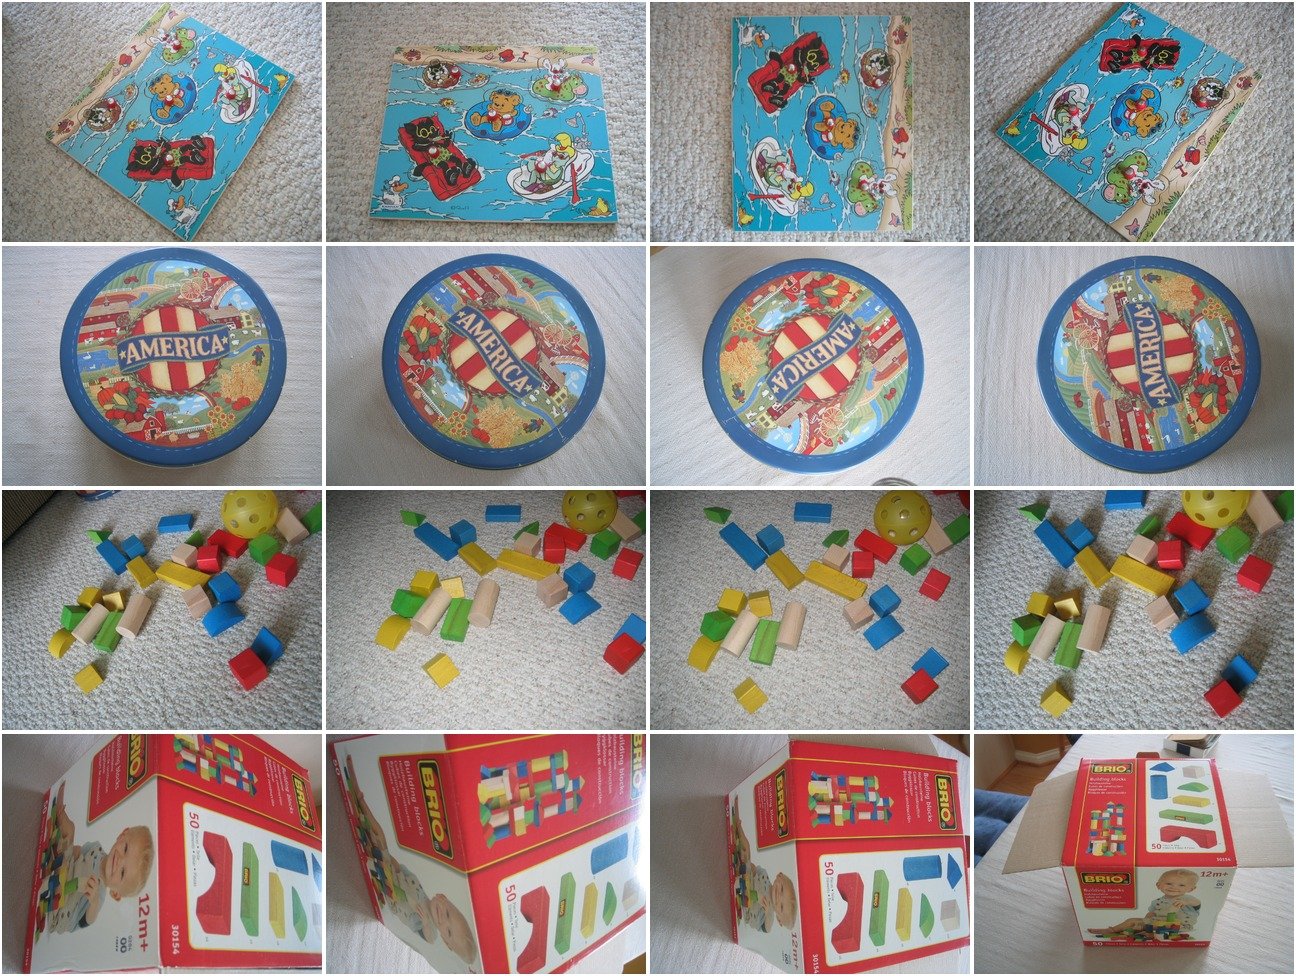
\includegraphics[width=0.9\linewidth]{chapter_firearm_ukb_images.jpg}
	\caption{UKB 数据集中一些示例图片}
	\label{fig:ukb_images}
\end{figure}

\section{图像收集与清理}\label{sec:image_collect_clean}
\subsection{图像的收集}
为了建设我们的枪支数据库,首先我们需要找到一些关键词,我们从一些论坛以及网站搜集了一批枪支名称的关键词。由于一个枪支可能会有很多的不同的型号以及很多仿照的型号,例如,根据维基百科\footnote{\url{https://en.wikipedia.org/wiki/M16_rifle}}, \emph{M16} 这个枪支就有至少三种不同的型号,分别为 \emph{M16A2}, \emph{M16A3}, \emph{M16A4},同时也有一些仿照的枪支,例如 \emph{XM177}。因此有必要处理收集到的关键词列表,去掉重复的关键词。我们认真审查了得到的关键词列表,确保一个枪支和它的不同型号以及仿照枪支不同时出现。经过人工的过滤以后,我们总共得到了 167 个关键词,这些关键词对应着不同的枪支类型,如「来复枪」,「手枪」,「散弹枪」等。

在得到这些枪支名称关键词以后,我们使用谷歌图像搜索引擎\footnote{\url{https://images.google.com/}},把这些关键词作为查询,提交到搜索引擎。对于每一个关键词,由于对应的枪支类型流行程度不同,因此返回的结果数目也不同,我们使用图片爬虫下载其中 300 -- 500 张图像作为初步的结果。

\subsection{图像的清理}
完成图像的收集以后,我们对图像进行了清理。我们主要去掉了以下几类图片:
\begin{itemize}
\item 损坏的图片(由于下载时候出现的错误)
\item 灰度图片(grayscale images)
\item 最小边小于 128 的小图片
\item 非 JPEG 格式的图片(GIF,TIFF,PNG 等格式)
\end{itemize}

经过图像清理过程,我们总共得到了 62642 张图片,在后续过程中,我们将对这些图片进行人工标注,然后进行评分与过滤,最后得到最终的枪支图片数据库。
\begin{figure}[t]
	\centering
	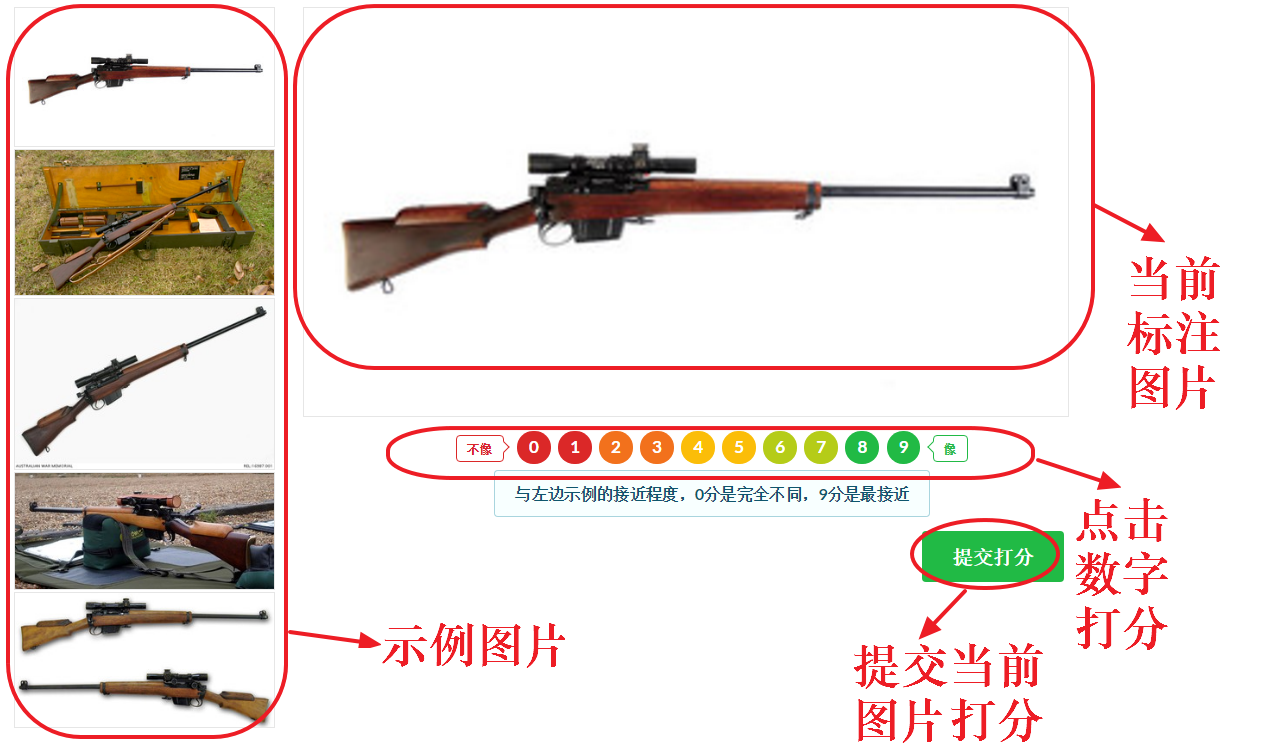
\includegraphics[width=0.9\linewidth]{chapter_firearm_ol_label_system.png}
	\caption{在线图像标注系统的评分界面}
	\label{fig:online_label_system}
\end{figure}

\section{图像标注及质量评估和图像的过滤}\label{sec:image_label_filtering}

\subsection{图像标注}
尽管谷歌的图像搜索引擎根据我们提供的检索词搜索到的图片质量已经相对较高,但是不可避免地,利用检索词搜索到的图片还存在一定的噪声(也就是说,根据某个检索词抓取的图片仍有一部分并不是对应于该检索词),因此我必须要对每一类图片\footnote{我们把通过同一个查询关键词抓取的图片当作一类}进行人工的标注,找出真正属于该类的图片。为了达到这个目的,我们构建了一个简单的在线标注系统,标注人员可以通过网页化的界面 (Web Interface) 对图像进行打分,从而帮助我们找出真正有效的图片。我们的在线标注系统的简单界面如图~\ref{fig:online_label_system}所示。


对于每一类图片,我们实现会人工找出五张真正属于该类的示例图片,然后我们对标注者进行了培训,指导他们标注应该如何进行。在标注过程中,标注者会根据当前要标注的图片(图~\ref{fig:online_label_system} 右上部分)与该类的示例图片(图~\ref{fig:online_label_system} 左边)的相似程度,对要标注的图片打分,分数范围为 $[0,9]$(0 分代表当前图片与示例图片毫不相关,9 分代表当前图片与示例图片最相似)。我们总共使用了 5 名标注者参与标注工作,每名标注者独立对每一类的所有图片进行打分。因此,在标注人员完成图片标注任务后,对于每一类图片下的每张图片,我们都有 5 个评分。

\subsection{图像标注质量评估}

\begin{figure}[t]
	\centering
	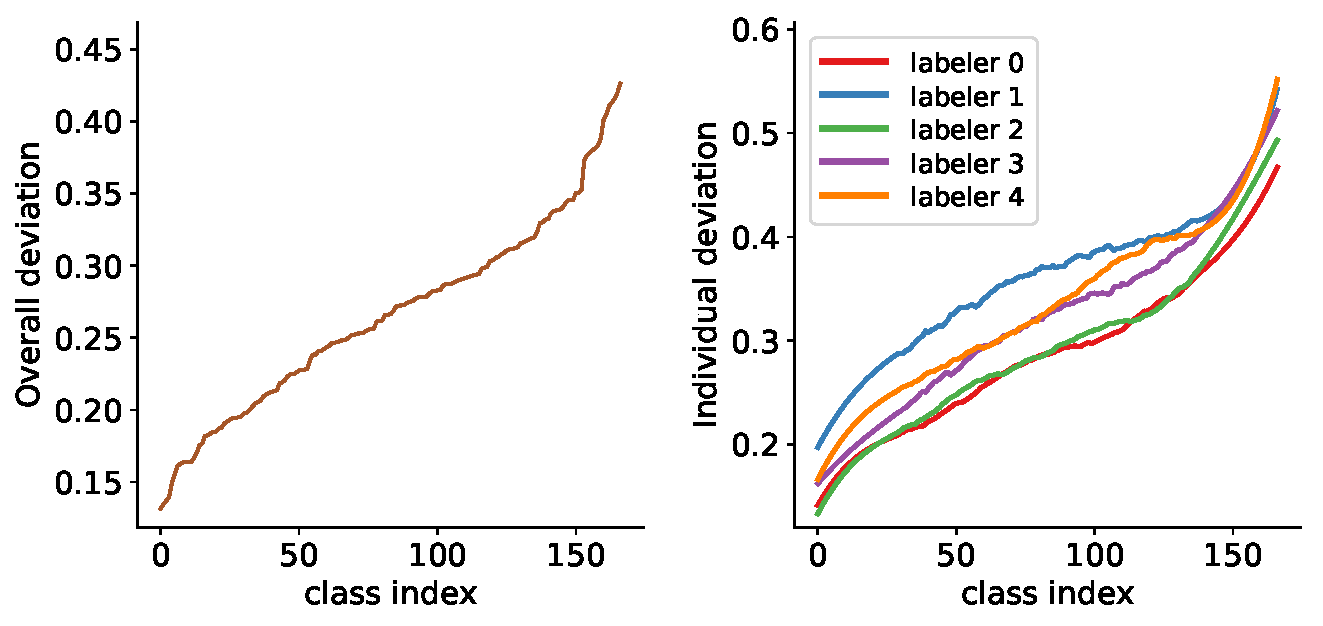
\includegraphics[width=\linewidth]{chapter_firearm_overall_individual_devi.pdf}
	\caption[枪支数据库打分数据的偏差统计信息]{枪支数据库打分数据的偏差统计信息。\textbf{左}:总体的偏差信息;\textbf{右}: 个人的偏差信息}
	\label{fig:deviation_info}
\end{figure}

不可避免地,不同的标注者的标注质量并不是相同的,标注质量的高低取决于很多因素,例如,标注者在标注过程中是否认真以及标注者对于相似的认识也可能有差异。为了给每一类下的每一张图片一个可靠的评分,我们必须科学地对标注者的标注质量进行评估。

首先,对于每一类图像,我们计算出不同打分者的打分之间的相关系数,我们用一个对称矩阵 $C$ 来表示相关性信息。矩阵 $C$ 的大小为 $5\times 5$,每个元素 $C[i,j]$ 代表第 $i$ 个标注者与第 $j$ 个标注者的评分之间的相关性。在理想情况下,两个标注者对某一类下面的图片评分肯定会有所不同 (某个图片的具体评分值可能会有不同),但是他们的打分相关性应该足够高,因此矩阵 $C$ 的每个元素都应该接近 1。如果一个标注者标注的质量不高,那么他/她的评分和其他人的评分之间的相关关系就会比较弱,我们可以据此定义每一类的总的偏差(overall diviation,OD)和个人偏差(individual deviation,ID)。对于某一类图片,总的偏差可以定义为:
\begin{equation}
OD = \frac{15 - \sum_{i=0}^{4}\sum_{j=i}^{4}C[i,j]}{15}\, ,
\end{equation}
对于标注者 $i$,个人偏差可以定义为:
\begin{equation}
	ID[i] = \frac{5 - \sum_{j=0}^{4}C[i, j]}{5}\, .
\end{equation}
在以上两个公式中,$C$ 是对应与某类的相关性矩阵。

在图~\ref{fig:deviation_info}中,我们展示了偏差信息的总体分布情况与个人分布情况:左图展示的总体的偏差分布情况,我们把偏差按照从小到大进行了排序;右图展示的是对应于每个人的偏差分布情况\footnote{为了滤除一些噪声,显示出趋势,我们对曲线进行了一定的平滑处理},和总体偏差采用了相同的类别编号顺序。一个标注者在某类上偏差越大,那么他在该类上的评分就越不可靠。从图~\ref{fig:deviation_info}中可以看出,标注者 1 在整体上有着最大的偏差(这意味着比较差的标注质量),标注者 3 和 4 相对来说,偏差较小,因此他们的标注质量较好,标注者 0 和 2 的总体偏差最小,因此他们的标注质量是最好的。

然后,我们统计了每个标注者在多少个类别上具有最大的个人偏差,这个指标可以用来衡量每个人的评分质量。在表~\ref{table:largest_devi_num}中,我们列出了统计数据。从中可以看出,在所有的 167 类中,标注者 1 在其中 93 类有最大的偏差值,这表明标注者 1 总体的标注质量很差;标注 3 和 4 在其中 33 类上有最大偏差值,这表明他们的标注质量中等,对于标注者 0 和 2,他们分别只在 167 类中的 9 类有最大的偏差值,这表明他们的标注质量是极其优秀的。
\begin{table}[!t]
	\centering
	\caption{每个标注者有最大的个人偏差的类别数目}
	\begin{tabular}{@{}llllll@{}}
		\toprule
		标注者编号	    &  0		& 1 & 2 & 3 & 4  \\
		\midrule
		数目 &  4 & 93 & 4 & 33 & 33 \\
		\bottomrule
	\end{tabular}
	\label{table:largest_devi_num}
\end{table}

\begin{figure}[!t]
	\centering
	\includegraphics[width=\linewidth]{chapter_firearm_dataset_aspect_ratio.pdf}
	\caption{Firearm14k 数据与其他数据库图片尺寸比值的分布}
	\label{fig:dataset_aspect_ratio}
\end{figure}

\subsection{图像过滤}
为了选出每一类的真正有效的图片,我们需要选出和给出的示例图片相似性得分高的图片。对于每一类别下的每张图片,我们使用五个标注者打分的加权平均分作为每张的图片的相似性得分。由于标注者 1 的评分质量太低,我们把标注者 1 的权重设为了 0,对于其他标注者,权重反比于他/她在多少类上有最大的个人偏差,这些权重之和为 1,我们最终使用的权重为

 \[w = [0.445, 0, 0.445, 0.055, 0.055]\]

对于每类下的每张图片,其最终的相似性得分 $s$ 为

\begin{equation}
s = \sum_{i=0}^{4}w_{i}s_{i}\, ,
\end{equation}

其中 $s_i$ 表示第 $i$ 个标注者对图片的评分。然后我们选择相似性得分在 6 分以上(含 6 分)的图片作为每类的有效图片,这些图片构成了我们的枪支数据库。

\begin{figure}[!t]
	\centering
	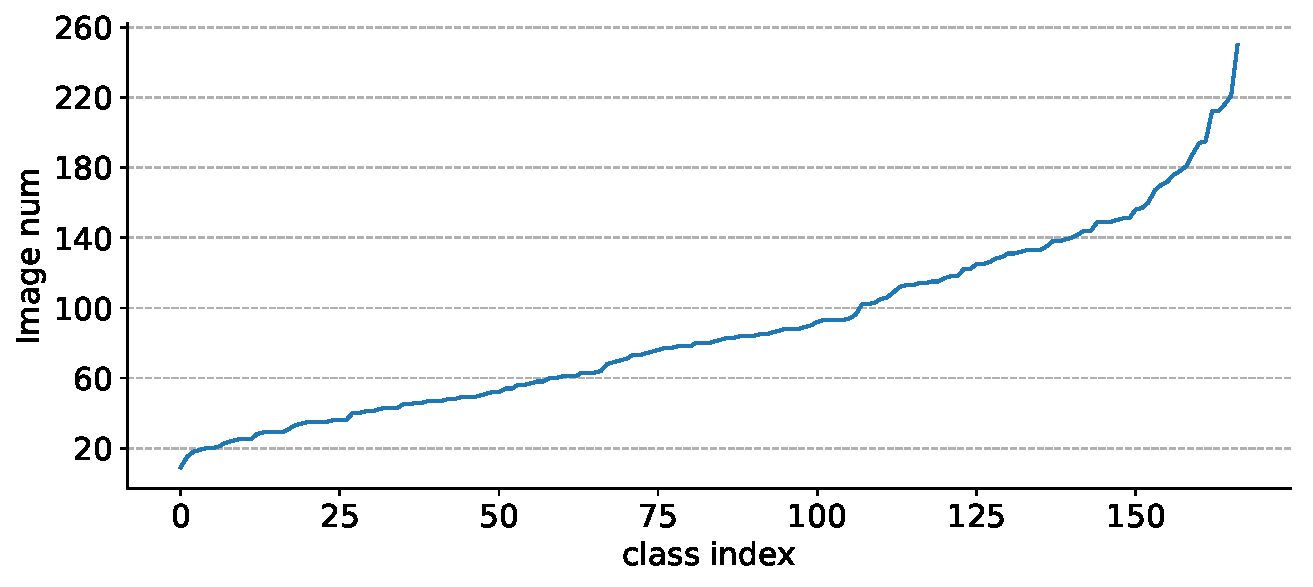
\includegraphics[width=\linewidth]{chapter_firearm_dataset_cls_img_num.pdf}
	\caption{枪支图像数据库各个类别图片数量}
	\label{fig:dataset_cls_img_num}
\end{figure}

\begin{table}[!t]
	\centering
	\caption[Firearm14k 数据库详细统计信息]{Firearm14k 数据库详细统计信息}
	\label{table:train_val_test_stat}
	\begin{tabular}{@{}llll@{}}
		\toprule
		          & 训练集 & 验证集 & 测试集 \\
		\midrule
		类别数目 & 107       & 20             & 40       \\
		图片数目 & 9628      & 1478           & 3649     \\
		查询图片数目 & --        & 39             & 80       \\
		图片库图片数目 & -- & 1438 &  3569 \\
		\bottomrule
	\end{tabular}
\end{table}

\section{数据库的划分与相关统计信息}\label{sec:dataset_stats}
最终,我们得到的枪支数据库含有 14755 张图片,这些图片来自 167 类不同类型的枪支,我们将该数据库命名为 Firearm14k。该数据库有几个值得注意的特点:

\begin{enumerate}
\item  该数据库具有高度不平衡 (imbalanced)的特点(图~\ref{fig:dataset_cls_img_num} 展示了数据库中各类的图片数目,按照图片数目从小到大排序),有的类别的图像包含的图片数目超过 200,还有一些类别图片数量大约只有 20 左右。

\item  由于该数据库包含很多长枪的图片,因此数据库中很多图片的长宽比都很大,在图~\ref{fig:dataset_aspect_ratio} 中,我们分别画出了 Firearm14k,Paris6k,Oxford5k 以及 ImageNet 数据库中图片尺寸的比例关系,对于每一个数据库,我们分别画出了宽和长的比($W/H$)以及长和宽的比例($H/W$)。Firearm14k 数据库由于长枪居多,所以宽长比和长宽比的分布呈现明显的两极化特点,两个分布交叉很少(见图~\ref{fig:dataset_aspect_ratio},左上),另外三个数据库由于长宽比不那么极端,两个分布呈现交错的状态。对于长宽比比较极端的数据库,如果在训练神经网络时把图片缩放为正方形,将会更严重地破坏图像的内容,保持图像长宽比显然是更好的选择。在第 \ref{chapter:double_margin}~章,我们通过实验也发现,保持图像的长宽比来训练网络,比固定图像长宽的方式得到的检索结果至少要高 2\%。

\item 该数据库中的图片是从真实世界中得到,图片中的枪支在尺度,拍照的视角,姿态,光照等因素的变化,背景也十分复杂,因而识别的难度很大。
\end{enumerate}

在图~\ref{fig:dataset_sample_images} 中,我们展示了一些随机选取自枪支数据库的示例图片,从图中可以看出,这些枪支图片中枪支的尺寸,拍摄的视角等变化千差万别,这给枪支图片的识别带来了很大的困难,也是我们试图解决的问题。

我们把数据库划分为训练集,验证集以及测试集,每个集合分别占总的图片量的大约 65\%,10\% 和 25\%,为了模拟真实的检索场景,三个集合的图片类别互不交叉 (具体做法是把 167 类图片随机划分为 3 个互不相交的类的集合,使得三个集合的图片数目占总图片量的比例接近预定的比例)。对于验证集和测试集,我们从每一类图片中随机选择了两张作为查询图片\footnote{验证集的查询图像中,有一张标注有错误,我们从查询图片中去掉了该图片},我们把剩余的所有图片作为分别作为验证集和测试集的搜索图像库。在表~\ref{table:train_val_test_stat}~中,我们列出了 Firearm14k 数据库的详细统计信息,表~\ref{table:train_val_test_stat} 第 2 行与第 3 行列出了三个集合的图片类别数目,图像数目。第 4 行和第 5 行列出了训练集以及验证集的查询图片数量以及对应的数据库图片数量。

\section{本章小结}
本章主要介绍了我们的枪支图片数据库的构建过程。首先,我们介绍了枪支图片的收集与清理,然后我们介绍了图像的标注过程,以及以相关性系数矩阵为基础,确定标注者的标注质量,进而得到图片的相似度分数,从而筛选出每一类真正有效的图片。最后,我们介绍了数据库的划分,列出了数据库的几个特点,并给出了数据库的详细统计信息。

\begin{figure}[!t]
	\centering
	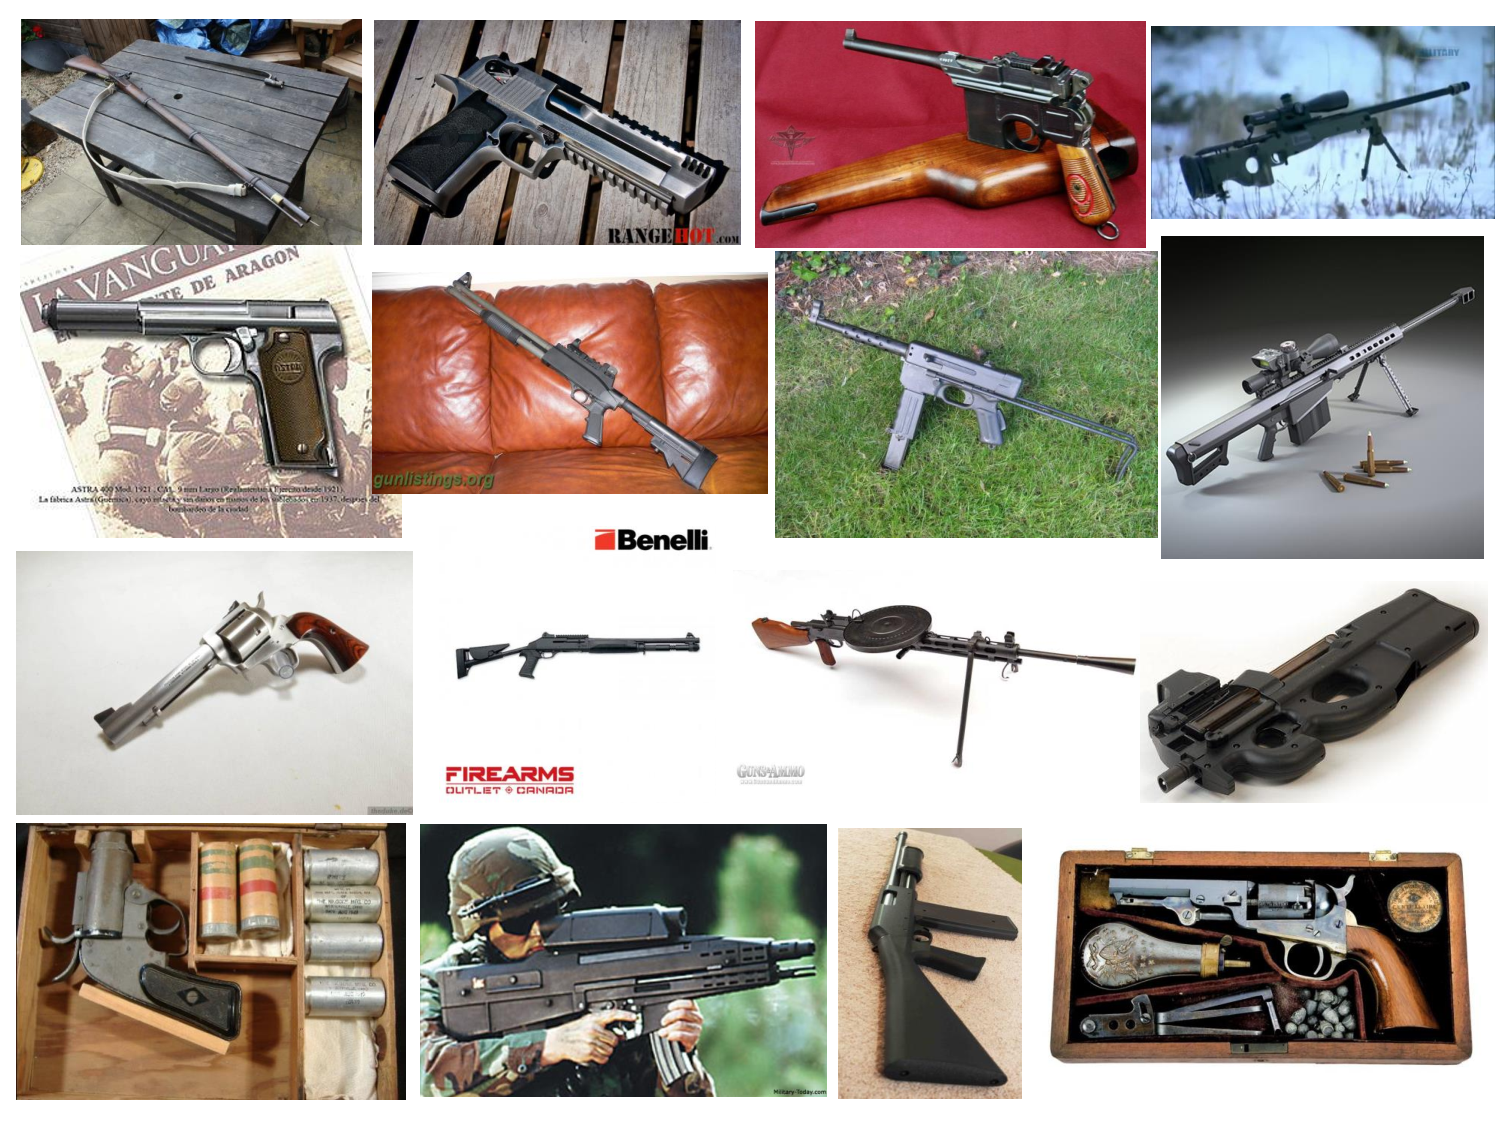
\includegraphics[width=\linewidth]{chapter_firearm_dataset_images.pdf}
	\caption{来自 Firearm14k 数据库的一些示例图片}
	\label{fig:dataset_sample_images}
\end{figure}



%!TEX root = ../Thesis.tex

\chapter{基于多尺度全卷积网络的图像实例检索方法}\label{chapter:mfc}
\section{引言}
图像检索是学术界以及工业界都非常关注的一个问题,按照检索的精细程度来分类,我们可以把图像检索方法分为两大类:第一类是基于类别的检索,在这种设定下,只要返回的某个搜索结果与查询图片属于同一大类(如「车」,「猫」,「狗」等),就认为该结果和查询图像是相关的;另外一类方法是精细检索,在本章中,我们研究的是图像实例级别的检索,在这种情况下,只有当返回的图片包含和查询图片相同的物体实例或者场景的情况下,我们才认为该图片与查询图片相关。在本章中,我们研究的基于实例的精细图像检索方法,尽管该问题是一个经典问题~\cite{Sivic2003VideoGA,Nistr2006ScalableRW,Philbin2007ObjectRW,Razavian2014CNNFO,Babenko2014NeuralCF,Tolias2015ParticularOR,Babenko2015AggregatingLD},前人的研究已经提出了很多的方法,但是由于图像中物体尺寸,方向,位置以及光照等条件影响,在不同图像上变化很大,该问题仍然是一个值得研究的问题。

图像检索领域的经典方法最常使用的是基于 SIFT 局部特征描述子~\cite{Lowe2004DistinctiveIF}的 bag of features (BOF)方法。通常为了提高检索的效果,研究者经常使用一些后处理技术,例如查询扩展~\cite{Chum2007TotalRA}以及空间验证~\cite{Philbin2007ObjectRW}。近些年来,由于卷积神经网络的流行,研究者也开始研究基于卷积神经网络的图像检索方法。他们的实验显示卷积神经网络在图像检索领域的有效性~\cite{Babenko2014NeuralCF,Razavian2014CNNFO,Tolias2015ParticularOR},他们发现,如果使用全局图像特征并且不使用后处理方法,基于卷积神经网络的方法和传统的 BOF 和局部聚合向量方法 (VLAD)~\cite{Jgou2010AggregatingLD}性能相似甚至超过这些方法。尽管使用卷积神经网络来进行图像特征表达取得了这些进步,一些影响特征有效性的潜在因素并未被详细研究,例如,图像缩放的策略,影响多尺度特征有效性的因素。研究清楚这些问题将帮助我们构建更加鲁棒与准确的检索系统。

我们详细研究影响图像特征有效性的一些因素,做出了一定的创新。不同于其他研究,我们使用了
全卷积神经网络,研究了图像尺寸对检索结果的影响,然后,我们研究了提取图像多尺度特征的不同设置对检索结果的影响,最后我们实验了不同的学习 PCA 与 白化矩阵用于特征降维的策略。结合我们的实验发现,我们提出了一种新的多尺度图像特征表达,该特征简洁而有效。我们在四个数据库上测试了提出的方法,大量的实验结果证明了我们提出的方法的有效性。

本章的结构组织如下:\ref{sec:mfc_factor_explaination}~节介绍我们提出的多尺度全卷积方法的几个构成要素,包括图像尺寸缩放方法,多尺度特征表达以及 PCA 与白化矩阵的使用。\ref{sec:mfc_experiment}~节给出各种因素对检索结果影响实验结果以及我们的方法和其他同类方法的对比结果。\ref{sec:mfc_related_work}介绍一些相关的工作。最后我们对本章的内容进行总结。

\section{基于多尺度全卷积网络的图像实例检索方法}\label{sec:mfc_factor_explaination}
\subsection{背景知识}
在本方法中,我们关注的是如何使用已有的神经网络模型,从中提出维度较低并且具有区分性的特征。对于图像 $I$,我们分别减去 RGB 三个通道均值,然后将图像送入神经网络,图像在神经网络中经过一系列卷积,池化以及非线性操作。神经网络某一层输出的特征图可以认为是图像的原始特征,基于此,我们可以进一步构建图像更复杂的特征。特征图构成了大小为 $C \times H \times  W$ 大小的张量,其中 $C$ 是特征通道的数目,$H$ 与 $W$ 是每个特征图的高和宽。我们用以下的公式代表特征图:

\begin{equation}
F=\{F_i\}, i=1,2,\ldots, C\, ,
\end{equation}
上式中,$F_i$ 代表第 $i$ 个特征图,最简单的图像特征可以用下面的公式表示:

\begin{equation}\label{eq:single_scale}
f = [f_1, f_2, \ldots, f_i, \ldots, f_C]^T\, ,
\end{equation}

其中,$f_i$ 是通过对特征图 $F_i$ 使用最大池化得到的。我们使用的特征图都经过 ReLU 操作,因此特征图每个元素都是非负的(我们也实验了经过 ReLU 操作之前的特征图,发现效果并不好)。在得到图像特征以后,我们对特征进行 PCA 以及白化处理。

\subsection{图像尺寸改变策略}\label{subsec:img_resize_strategy}
计算机视觉各个领域的研究者为了自己的研究目的,通常使用一些在 ImageNet~\cite{Russakovsky2015ImageNetLS} 上训练的模型~\cite{Krizhevsky2012ImageNetCW,Simonyan2014VeryDC,Szegedy2015GoingDW,He2016DeepRL},然后对这些模型进行一些改造以适应自己的研究。这些网络通常会对输入网络的图像尺寸有要求,为了满足网络对图像尺寸的要求,一些检索方面的工作~\cite{Gong2014MultiscaleOP,Babenko2015AggregatingLD}通常对输入图像进行变化,使得图像的长宽变成固定值。图像的缩放操作可能会导致图像中物体信息的丢失或者扭曲,因此从网络中提取的图像特征的区分性不强,检索效果变差。对于图像检索任务,我们认为最好保持图像原有的大小,直接把图像输入神经网络。我们研究了三种不同的图像大小改变的策略:
\begin{itemize}
\item 图像的长和宽都被变为固定值,这种策略用 \emph{two-fixed} 表示。

\item 图像的最小边为固定值,但是保持图像的长宽比不变,这种策略用 \emph{one-fixed} 表示。

\item 保持图像原尺寸,这种策略用 \emph{free} 来表示。
\end{itemize}

\begin{figure}[!t]
	\centering
	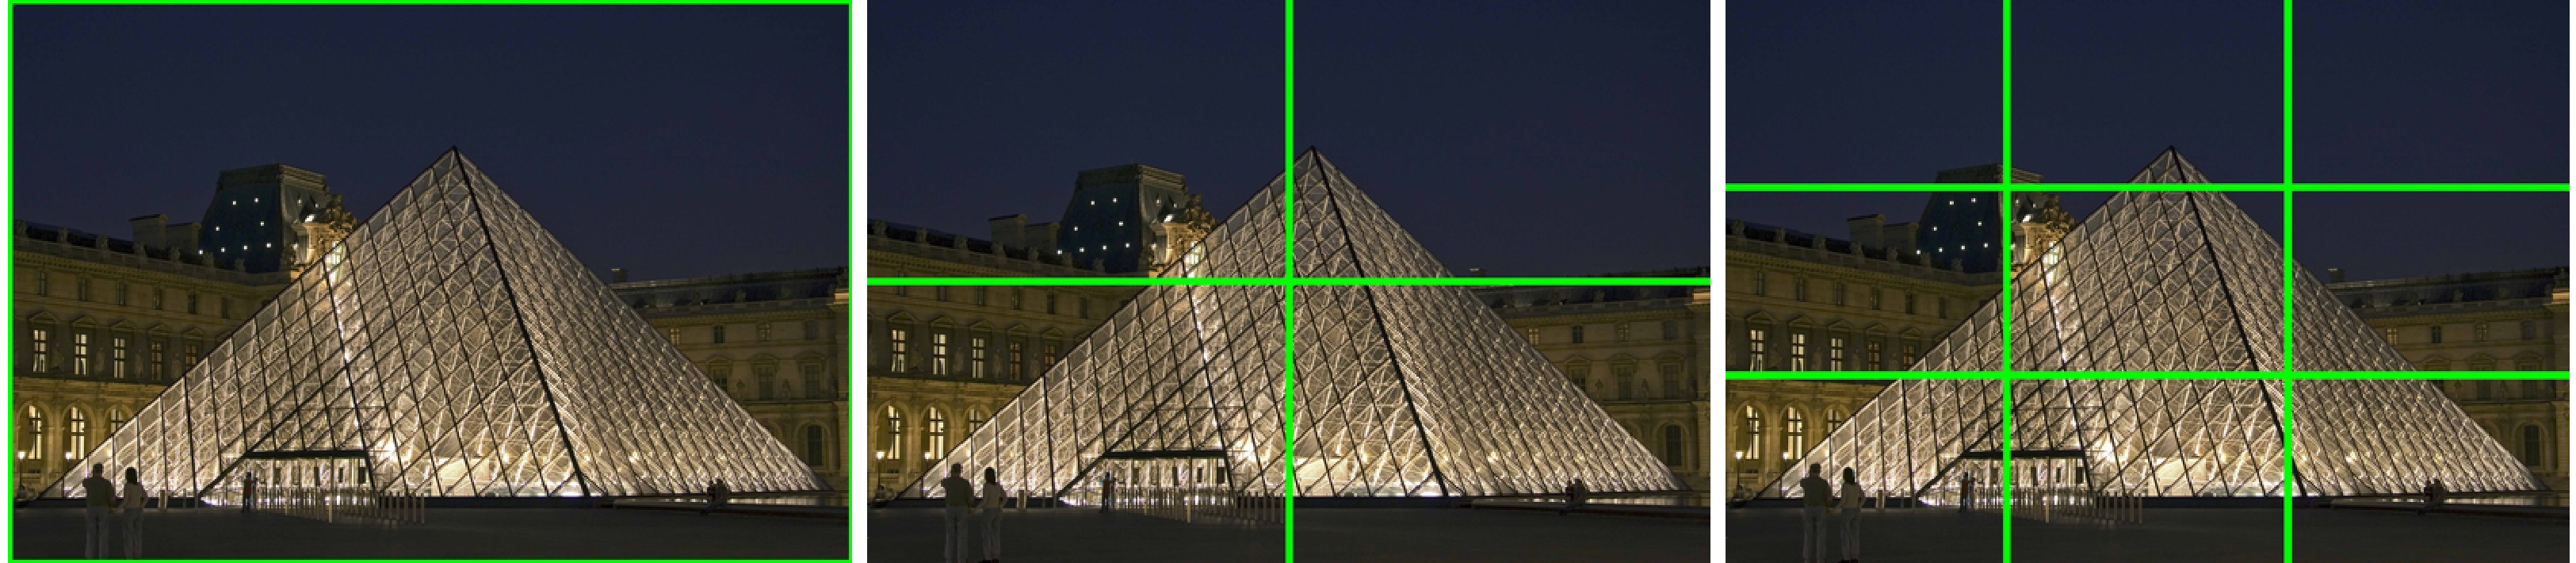
\includegraphics[width=\linewidth]{chapter_mfc_paris_3scale.pdf}
	\caption{图像的 3 尺度特征表示}
	\label{fig:img_multiscale_feature}
\end{figure}

\subsection{多尺度特征表达}\label{subsec:multiscale_img_repr}
不同于 SIFT~\cite{Lowe2004DistinctiveIF}等局部特征描述子,从神经网络提取的特征向量是全局描述子,编码的是图像的全局信息,因此得到的图像特征和图像的语义上的类别关系紧密但是缺乏一些局部以及细节信息,这些细节信息正是评价图像相似性所需要的。受一些多尺度图像特征表达工作~\cite{Lazebnik2006BeyondBO,He2014SpatialPP}的影响,我们试图把这种有效的特征表达方式与合适的图像尺寸改变策略结合在一起,得到具有区分性的特征。在我们的方法中,一张图像由 $L$ 个不同尺度的图像特征金字塔表示,在每个尺度,图像被分为多个互相重合或者不重合的区域,图~\ref{fig:img_multiscale_feature}展示了一张图像 3 尺度表示的示意图。然后我们计算每个小区域的特征表达,并把来自同一尺度的局部特征表达结合起来形成每个尺度的特征。最后我们把每个尺度的特征结合起来,$l_2$ 归一化作为图像最后的特征。

我们试验了三种不同的用来结合局部特征以及不同尺度特征的方法。第一种方法和 He 等提出的空间金字塔~\cite{He2014SpatialPP}相似,来自不同尺度的所有区域特征被 $l_2$ 归一化,然后被拼接成一个特征向量,因此该向量的维度很高,为 $N\times C$,其中 $N$ 是所有来自不同尺度的小区域的个数,$C$ 是特征通道的个数。第二种方法中,区域特征求和并被归一化以后形成尺度级别的特征,然后尺度级别的特征被拼接起来形成图像特征,因此这个特征的维度为 $L \times C$,其中 $L$ 代表尺度的个数。在第三种方法中,区域级别的特征被加起来,然后归一化形成尺度特征,然后尺度特征随即被求和、归一化形成图像的特征表达,图像特征维度为 $C$(特征通道的个数)。

如何有效计算图像各区域的特征也是需要考虑的问题,如果我们将每个图像小块分别送入神经网络来提取特征,计算一张图像特征需要消耗大量的时间,这对于图像检索应用是不现实的。受 ROIpooling~\cite{Ren2017FasterRT}以及 R-MAC(regional maximum pooling of activations) 方法~\cite{Tolias2015ParticularOR}启发,如果我们假设图像区域与特征图对应区域是线性映射关系,那么我们就可以有效地计算图像区域特征,而不用把图像小块重新输入网络。在实验部分,我们实验了不同的提取多尺度特征的设置,报告不同设置得到的特征的检索性能并给出我们的分析。

\subsection{特征降维与白化}
主成份分析法(PCA)是一种常用的有效的特征降维方法,该方法可以使特征的各个分量之间相互独立,白化(whitening)则是使得特征均值为 0,方差为 1。之前的工作~\cite{Babenko2014NeuralCF}已经表明经过 PCA 和 白化以后,特征的检索效果将会提高。在本章中,我们也给出我们的一些发现。

\section{实验}\label{sec:mfc_experiment}
\subsection{实现细节}
我们使用开源深度学习框架 Caffe~\cite{Jia2014CaffeCA}来进行我们所有的实验。我们使用的模型是非常流行的 VGG19 模型~\cite{Simonyan2014VeryDC},该模型是在 ImageNet~\cite{Russakovsky2015ImageNetLS} 分类数据上训练得到的。在实验中,我们使用的特征图来自于网络的最后一层卷积层的输出。

由于原有的 VGG 模型只能接受固定大小的图像输入,这种方式对于需要提取图像特征的检索任务来说,并不是最好的方式。为了使网络能够处理各种大小与长宽比的图像并且测试我们提出的图像尺寸改变的策略,我们把网络变成了全卷积的网络,使得网络能够接受任何大小与长宽比的图像。

\subsection{评价指标与数据库}

\noindent\textbf{(1)评价指标}

图像检索领域两个最基本的指标是准确率(precision)与召回率(recall),准确率指的是返回的结果中,有效的样本占所有返回结果的比例,随着返回结果的增多,准确率通常会降低,常用的还有前 K 个返回结果的准确率,用 precision@k 表示;召回率则指的是返回的结果中,有效的样本占所有有效样本的比例,随着返回结果的增多,召回率通常会上升,同样地,研究者也常使用前 K 个返回结果的召回率,用 recall@k 表示。准确率与召回率是考虑系统性能的两个重要指标,一般来说,准确率高的时候,召回率会比较低,而召回率高的时候,准确率通常又比较低(极端情况就是返回所有的样本,召回率 100\%,但是准确率很低),因此一个好的检索方法必须同时在准确率与召回率上都取得较好的结果,在两个指标上取得平衡。

对于单个查询来说,为了综合反映检索算法的性能,通常并不单独使用准确率和召回率,二是使用综合性的指标,最常使用的一个指标是平均准确率(average precision,简称 AP),该指标同时考虑准确率与召回率,实际上计算的是准确率-召回率曲线下面的面积,用公式表示该指标如下:

\begin{equation}\label{eq:average_prec}
AP = \sum_{k=1}^{n}P(k)\Delta r(k)
\end{equation}

公式\ref{eq:average_prec}中,$P(k)$ 代表 precision@k,$\Delta r(k)$ 代表从 $k-1$ 到 $k$,召回率的变化。

评价检索算法在某个数据库上的性能,常用的评价指标是 mean average precision(简称 mAP),该指标指的是一个数据库上所有查询对应的平均准确率(AP)的均值,用公式表示如下:

\begin{equation}\label{eq:mean_avg_prec}
\text{mAP} = \frac{\sum_{q=1}^{Q}AP(q)}{Q}
\end{equation}

公式\ref{eq:mean_avg_prec}中,$AP(q)$ 代表某个查询 $q$ 对应的平均准确率,$Q$ 代表所有查询的数目。

\noindent\textbf{(2)数据库}

\textbf{Oxford5k} 数据库\cite{Philbin2007ObjectRW}包含了 5062 张从 Flickr 上抓取的 Oxford 建筑图片。该数据库总共包含 55 个查询图像,每个查询图像包含有具体查询区域的坐标,在实验中对于每一幅查询图像,我们使用了两种查询,分别是 \emph{full-query}(使用整个查询图像) 和 \emph{cropped-query}(使用坐标指定区域内的图像)。在该数据库上的评价指标为 mAP。

\textbf{Paris6k} 数据库\cite{Philbin2008LostIQ}包含了 6412 张来自巴黎的建筑图片\footnote{按照惯例,该数据有 20 张被损坏的图片被去掉,因此实际图片数量是 6392。}。与 Oxford5k 数据库类似,该数据库也包含了 55个 查询图像,同时附带每个图像对应的感兴趣区域的坐标。在这个数据库上的评价指标是 mAP。

\textbf{Oxford105k} 数据库包含了的是 Oxford5k 数据库的图片以及额外 100,000 张来自 Flickr 的图片\footnote{有一张损坏图片 \verb+oxc1_100k\portrait\portrait_000801.jpg+ 被移除}~\cite{Philbin2007ObjectRW}。这 100,000 张
图片与 Oxford5k 没有相同的图片,被用来作为干扰图片,主要是为了验证数据库规模扩大时的算法的性能。在这个数据库上的评价指标与 Oxford5k 完全一致。

\textbf{UKB} 数据库\cite{Nistr2006ScalableRW}总包含了 2550 个物体的 10200 张照片,每个物体 4 张照片。实验时,每张图片被用作查询图片去查询其他图片(包含该图片本身),在这个数据上的评价指标比较特殊,用返回的前四张图片与查询图片相似的平均数目来衡量,是区间 $[0,4]$ 上的一个数,也就是 $4\times recall@4$。

\subsection{实验结果与分析}
在本部分,我们对不同的因素对检索结果影响进行了详细的实验,并给出相应的分析。


\noindent\textbf{(1)图像尺寸变化对检索的影响}

我们对\ref{subsec:img_resize_strategy}节给出的三种图像尺寸变化的策略进行了实验,对于 \emph{two-fixed} 和
\emph{one-fixed} 策略,由于图像的尺寸可以选择多种,我们使用网格搜索来找到性能最好时对应的图像尺寸。我们发现,总体来说,增加图像的尺寸,对于 \emph{full-query} 或者 \emph{cropped-query} 这两种情况,都会提升检索的效果,试验结果如表~\ref{table:image_size_impact}所示,表中括号后面的数字表示取得最好的 mAP 时使用的图像尺寸。从表上可以看出,对于 \emph{cropped-query} 这种情况,\emph{free} 策略能够有效地提升检索的性能,对于 \emph{full-query},\emph{free} 与 \emph{one-fixed} 策略则比较接近,但检索的效果都要好于 \emph{two-fixed} 策略。我们可以看出 \emph{one-fixed} 策略此时要稍高于 \emph{free} 策略,但是 \emph{one-fixed} 情况下,图像最小的边长度被固定在 800,这种设置将大大增加提取特征所需要的计算时间,因为数据库中大部分图像最小尺寸都要小于 800(在表\ref{table:min_size_distribution}中,我们列出不同数据库中的图像最小边尺寸的统计信息)。采用 \emph{free} 方式,我们减少特征提取提取时间,并且能够取得很好的检索结果。

实验表明,改变图像的长宽比 (对应 \emph{two-fixed} 策略)对图像信息的干扰最大,因此检索的精度有明显的下降。\emph{one-fixed} 策略虽然没有改变图像的长宽比,但是由于图像尺寸的变化,仍然有一部分信息的丢失。\emph{free} 方式能够编码图像未经扭曲与破坏的信息,因而得到的特征效果更好,能够取得更好的检索结果。

\begin{table}[!t]
	\centering
	\caption{不同图像尺寸变化策略之间的比较}
	\label{table:image_size_impact}
	\begin{tabular}{lll}
		\toprule
		方法		    & full-query			& cropped-query \\
		\midrule
		\emph{two-fixed}		&		55.5 (864)		& 	38.7 (896)	\\
		\emph{one-fixed}		&		59.0 (800) 		&	39.3 (736)\\
		\emph{free}				&		58.0	 		&	52.6 	\\
		\bottomrule
	\end{tabular}
\end{table}

\begin{table}[!t]
	\centering
	\caption{不同数据库中图像最小尺寸落在各个区间的比例($s$ 代表最小尺寸)}
	\label{table:min_size_distribution}
	\begin{tabular}{llll}
		\toprule
		Dataset & $s\leq 500$ & $500<s\leq 800$&  $s>800$ \\
		\midrule
		Oxford5k & 0.87 & 96.86 & 2.27 \\
		Paris6k & 1.30  & 95.59 & 3.11 \\
		Flickr100k & 1.49 & 93.91 & 4.60\\
		UKB & 100 & 0 & 0 \\
		\bottomrule
	\end{tabular}
	\end{table}

\noindent\textbf{(2)图像的多尺度特征表达}

首先我们通过实验比较了\ref{subsec:multiscale_img_repr}节提出的区域特征以及尺度特征融合策略,实验结果表明前两种特征融合策略效果不如第三种策略。如果使用第一种策略,检索效果比第三种策略要低 41\%。同时,使用前两种方法得到的图像特征维度(维度至少为 1500 维)也要高于第三种策略(特征维度为 512 维)。高纬度特征也会使得检索时间变长,综合考虑这些,我们采用第三种方式来融合不同的特征。

我们进行了大量实验来确定多尺度方法最好的配置,实验结果列于表~\ref{table:multiscale_exp_result}中。在表中,「overlap」用来指示每个尺度的各个图像区域是否有重叠部分,「s2」和「s3」表示重叠发生了尺度 2 和 3。「weighing」表示各个尺度特征融合的时候,是否采用了不同的权重或者相同的权重。「version」则表示每个尺度使用不同数目的图像块。
\begin{table}[!t]
	\centering
	\caption{不同设置下多尺度特征检索结果对比}
	\label{table:multiscale_exp_result}
	\begin{tabular}{@{}lllllll@{}}
		\toprule
		&   scale &  overlap   &  weighing  & version &     full    &    cropped    \\
		\midrule
		(a1) &   2   & \texttimes & \texttimes &    -    &     63.5      &     59.0      \\
		(a2) &   2   & \texttimes & $\checkmark$ &    -    &     63.9      &     61.0      \\
		\midrule
		(b1) &   3   & \texttimes & \texttimes &    -    &     64.2      &     60.9      \\
		(b2) &   3   & \texttimes & $\checkmark$ &    -    &     62.6      &     61.0      \\
		(b3) &   3   &     s2     & \texttimes &    -    &     64.8      &     60.8      \\
		\midrule
		(c1) &   4   &     s3     & \texttimes &   v1    &     65.1      &     61.4      \\
		(c2) &   4   &     s3     & $\checkmark$ &   v1    &     64.8      &     60.7      \\
		(c3) &   4   &   s2,s3    & \texttimes &   v1    &     65.5      &     60.8      \\
		(c4) &   4   &   s2,s3    & \texttimes&   v2    &     65.9      &     61.5      \\
		(c5) &   4   &   s2,s3    & $\checkmark$ &   v2    &     65.4      &     61.2      \\
		(c6) &   4   & \texttimes & \texttimes &   v3    &     64.5      &     61.3      \\
		(c7) &   4   &     s3     & \texttimes&   v3    &     65.8      &     62.2      \\
		(c8) &   4   &   s2,s3    & \texttimes&   v3    & \textbf{66.3} & \textbf{62.6} \\
		\bottomrule
	\end{tabular}
\end{table}

首先,我们研究了尺度的个数对检索精度的影响。当使用的尺度数目分别为 2 和 3 时,我们使用的每个尺度的区域数目分别为 $\{1\times1, 2\times2\}$ 和
$\{1\times1, 2\times2, 3\times3\}$。对于尺度为 4 的情况,我们使用三种不同版本的区域数目:对于「v1」,「v2」以及「v3」,所使用的图像区域数目分别为 $\{1\times1, 2\times2, 3\times3, 4\times4\}$,$\{1\times1, 2\times2, 3\times3, 5\times5\}$ 和 $\{1\times1, 2\times2, 3\times3, 6\times6\}$。表~\ref{table:multiscale_exp_result}中 (a1)、(b1)、(c6) 三行列出了分别使用 2, 3, 4 个尺度表示数据图像特征得到的检索结果。很显然,尺度数目的增加也使得检索结果性能变好,特别是对于\emph{cropped-query},检索的结果提高了 3.9\%。

接着,我们也研究给不同的尺度的特征加权融合是否会提升检索的效果。我们使用的不同的尺度的特征加权融合方式类似空间金字塔匹配方法~\cite{Lazebnik2006BeyondBO},也就是说,给来自粗糙尺度上特征更少的权重,给来自精细尺度的特征更大的权重。假设当前总共有 $L$ 个尺度,对应的特征为 $f^1, f^2, \ldots, f^L$,则图像特征 $f$ 计算方式为:

\begin{equation}
f = \frac{1}{2^{L-1}}f^1 + \sum_{i=2}^{L}\frac{1}{2^{L-i+1}}f^i\, .
\end{equation}
关于空间金字塔匹配方法更多的细节,可以参见 Labebnik 等的论文~\cite{Lazebnik2006BeyondBO}。比较 (a1) 和 (a2) 行的结果,看起来似乎加权的方式可以提升检索的性能。我们做了更多的实验,发现随着尺度数目的提高,加权方式来求图像特征并不能提高检索的性能,反而得到了更差的结果,例如,比较 (b1)(b2) 两行的结果,或者比较 (c1)(c2) 两行。这里的结果表明,深度学习提取的特征和传统的特征描述子不同。因此当我们使用对传统的 SIFT 特征有效的方式时,应该有所警惕~\cite{Babenko2015AggregatingLD}。基于这里的实验结果,我们在计算图像特征时,不使用权重不同的策略。

最后,我们研究了同一尺度下不同图像区域重叠(overlapping)是否会提高检索的结果。对于不同尺度数目,我们在一个或者两个尺度下使用重叠的策略。对于行 (b1)(b3) 和 (c1)(c3),我们观察到使用重叠的方式提高了 \emph{full-query} 情况下的结果,但是却降低了 \emph{cropped-query} 情况下的结果。但是对于尺度数目为 4 ,版本是「v3」的情况(比较 (c7)(c8)),我们可以观察到对于 \emph{full-query} 和 \emph{cropped-query},检索结果都有所提高。因此计算最终的图像特征时,我们在尺度 2 和 3 使用了重叠的策略。


\begin{figure}[!t]
	\centering
	\begin{subfigure}{.5\columnwidth}
		\centering
		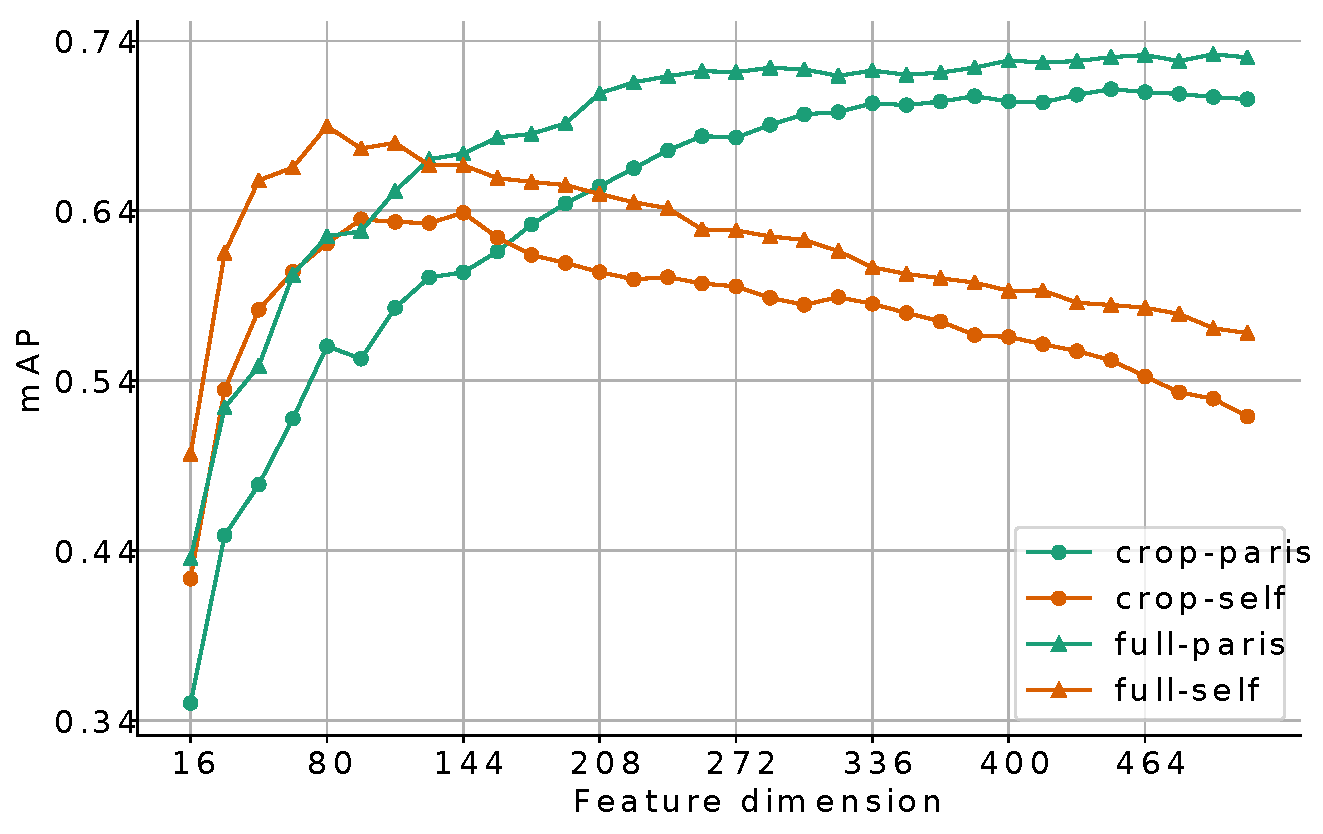
\includegraphics[width=\linewidth]{chapter_mfc_oxford_pca_other_self.pdf}
		\subcaption{Oxford5k}
	\end{subfigure}%
	\hfill
	\begin{subfigure}{.5\columnwidth}
		\centering
		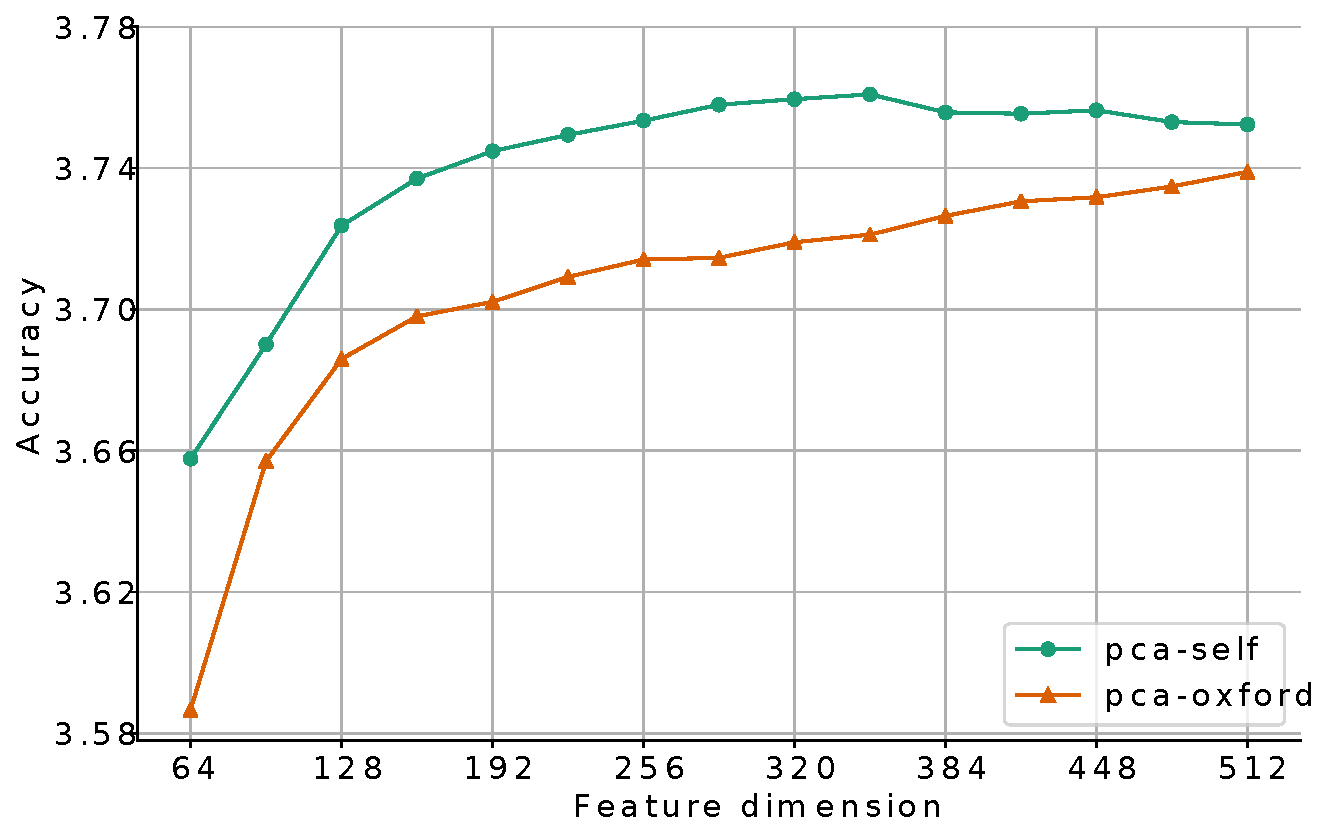
\includegraphics[width=\linewidth]{chapter_mfc_ukb_pca_other_self.pdf}
		\subcaption{UKB}
	\end{subfigure}
	\caption{学习 PCA 与白化矩阵的方式对不同数据库检索结果的影响}
	\label{fig:pca_self_other_exp}
\end{figure}

\noindent\textbf{(3)主成份分析与白化方法}

我们在 Oxford5k 以及 UKB 数据库上进行了 PCA 与白化对检索影响的实验。对于 Oxford5k 数据库,我们分别从 Oxford5k 数据库本身(我们称为「pca-self」)或者从 Paris6k 数据库(我们称为「self-paris」)学习 PCA 与白化矩阵;对于 UKB 数据集,PCA 与白化矩阵则从 UKB 本身(称为「pca-self」)或者从 Oxford5k 上(称为「pca-oxford」)学习得到。我们发现,对于 Oxford5k 数据库,如果从 Paris6k 上学习 PCA 与白化矩阵,检索结果将会提高。但是 UKB 数据库,由于它和 Oxford5k 数据库和 Paris6k 数据库风格不同,从 Oxford5k 数据库学习到的 PCA 与白化矩阵反而对检索结果有害。图~\ref{fig:pca_self_other_exp}清楚展示了这种不同。同时,对于 Paris6k 数据库,我们也有同样的结果,当使用从 Oxford5k 数据库学习到的 PCA 与白化矩阵时,检索的结果也会有所提升。


\subsection{与其他方法的对比} \label{subsec:mfc_compare_soa}
基于前面的实验结果以及我们的对不同影响因素的分析,我们提出了 \textbf{MFC} 方法 --- 一种多尺度全卷积的图像特征表达方法。对于一张图像,我们不对它进行缩放(\emph{free} 的方式),直接输入到神经网络,然后我们从神经网络的最后一层卷积层的输入的特征图的基础上,提取 4 尺度图像特征表达。在多尺度特征表达中,我们使用最大池化处理特征图,并且使用了区域重叠的策略,我们把区域级别的特征加起来形成尺度特征并归一化,然后把各个尺度的特征求和得到图像特征,再一次归一化。之后,我们学习 PCA 与白化矩阵,对图像特征进行降维。对于不同待测数据库,我们用来学习 PCA 和白化矩阵的数据库分别如下:对于 Oxford5k 及 Oxford105k,我们使用的是 Paris6k;对于 Paris6k 和 UKB,我们使用数据库分别是 Oxford5k 以及 UKB。经过 PCA与白化处理的特征,被再一次归一化,得到最终的特征,这个特征用来报告各种方法的性能。

我们把提出的方法与一些主流的方法进行了比较,这些方法都使用了较低维度的特征,并且没有使用复杂的后处理方法,如几何重排序~\cite{Philbin2007ObjectRW}以及查询扩展~\cite{Chum2007TotalRA}。我们使用了不同的特征维度,实验结果见表~\ref{table:mfc_compare_with_soa},「D」代表特征的维度,「full」与「cropped」分别代表 \emph{full-query} 以及 \emph{cropped-query}。和其他方法相比,在不同的特征维度下,我们的方法都取得了不错的结果。

\begin{table}[!t]
	\centering
	\caption{与其他方法的对比}
	\label{table:mfc_compare_with_soa}
	\begin{tabular}{lllllllll}
		\toprule

		\multirow{2}*{方法}   & \multirow{2}*{D} & \multicolumn{2}{c}{Oxford5k} & \multicolumn{2}{c}{Paris6k} & \multicolumn{2}{c}{Oxford105k} & \multirow{2}*{UKB} \\

		\cmidrule(lr){3-4}	\cmidrule(lr){5-6} \cmidrule(lr){7-8}
		 &                  & full & cropped               & full & cropped              & full & cropped                 &                    \\
		\midrule
		Razavian et al. \cite{Razavian2014CNNFO}              & 256              & 58.9 & -                     & 57.8 & -                    & -    & -                       & 3.65               \\
		SPoC \cite{Babenko2015AggregatingLD}                     & 256              & 58.9 & 53.1                  & -    & -                    & 57.8 & 50.1                    & 3.65               \\
		Neural codes\cite{Babenko2014NeuralCF}                   & 512              & 55.7 & -                     & -    & -                    & 52.2 & -                       & 3.56               \\
		R-MAC \cite{Tolias2015ParticularOR}                      & 512              & -    & 66.8                  & -    & 83.0                 & -    & 61.6                    & -                  \\ \midrule
		Ours                                                     & 256              & 72.2 & 68.4                  & 82.5 & 83.4                 & 68.0 & 62.9                    & 3.75               \\
		Ours                                                     & 512              & 73.0 & 70.6                  & 82.0 & 83.3                 & 68.9 & 65.3                    & 3.75               \\
		\bottomrule
	\end{tabular}
\end{table}

\section{相关工作}\label{sec:mfc_related_work}
Labebnik 等人~\cite{Lazebnik2006BeyondBO}提取使用空间金字塔匹配(简称 SPM)来编码图像的空间信息,在该方法中,可以用多个尺度的金字塔来表示一张图像。来自不同的尺度的特征被结合在一起形成图像的特征,在特征融合的时候,来自精细尺度的特征得到了更多的权重,来自粗糙尺度的特征得到了更少的权重。He 等人~\cite{He2014SpatialPP}提出空间金字塔池化方法(简称 SPP),该方法把神经网路最后一层卷积层输出的特征图划分为不同尺度的金字塔,每个尺度下的区域特征,以及各个尺度的特征被拼接在一起,形成了图像的特征。在我们的工作中,我们也探索了这两种方式是否可行,我们发现使用更简单的特征聚合方式反而取得了更好的结果。

本章采用的是直接提取特征不经过微调的方式来提取图像特征,在这方面有一些喝我们的方法相关的工作。Tolias 等人~\cite{Tolias2015ParticularOR}以及 Babenko 等人~\cite{Babenko2015AggregatingLD}提出使用神经网络的最后一层卷积层的输出作为图像特征,他们分别采用了不同的特征池化方式。Tolias 等人还提出使用一种多尺度的特征表达方式,被称为 R-MAC(regional maximum activation of convolutions),特征图被分为 3 个不同的尺度,每个尺度有一些相互重叠的区域构成,每个尺度的区域个数由原图的长宽比决定。在我们的方法里,我们使用了更简单的策略,每个尺度下区域的个数是固定的,区域的大小根据图像长宽比不同而变化。另外这些工作也没有讨论图像尺寸对检索结果的影响以及该如何学习 PCA 和白化矩阵,才能提升检索的性能。

\section{本章小节}\label{sec:mfc_conclusion}
在本章中,我们介绍了所提出多尺度全卷积的图像特征提取方法。前人工作没有详细地探讨各种因素对检索结果的影响,在本工作中,我们对图像尺寸缩放的策略,多尺度提取特征的方式,以及 PCA 和白化矩阵学习这三个重要的因素进行了研究,并进行了大量的实验,分析三个因素对检索的影响,在此基础上提出了我们的多尺度全卷积的图像特征提取方法。我们在四个数据库进行了实验,实验结果也表明我们提出的方法取得了良好的效果。

%!TEX root = ../Thesis.tex

\chapter{基于双阈值对比损失函数的枪支图像检索方法}\label{chapter:double_margin}

\section{引言}
在社交媒体上,经常会有用户把枪支等敏感图片上传到自己的主页,这些图片可能助长非法的枪支交易~\cite{Drange2016,MELE2016FacebookBG},也可能引发其他用户的不适,因此某些类型的枪支图片(如机关枪,自动步枪等)需要适当的监管与控制~\cite{Hsu2018Bumble},如果普通用户在社交媒体上展示不能随意购买的枪支,这可能预示着非法的交易。另外,在取证科学上,取证人员有时也需要根据枪支的图片确定枪支的具体品牌与型号,由于枪支类型的繁杂,除非取证人员经过专门的训练,否则很难从庞大的枪支数据库准确找到具体的枪支类型。基于图像检索的任务能够有效地帮助解决以上的需求,我们只需要使用已经训练好的模型提取图像的特征,然后计算图像特征之间的距离,采用最近邻方法就可以确定具体的枪支类型。

在本章中,我们研究枪支图像的精细(fine-grained)检索问题,也就是说,给定一个检索的枪支图像,我们的方法需要从数据库找到和给定图像属于同样精细类别的图片~\cite{Song2016DeepML,Wang2017DeepML}。图像精细检索任务相当困难,因为不同于行人再识别(ReID)~\cite{Zhao2013UnsupervisedSL,Li2014DeepReIDDF}与人脸识别~\cite{Wen2016ADF,Taigman2014DeepFaceCT}等任务,图像精细检索任务中使用的图片都是非对齐的(un-aligned)图片,也就是说,在训练和测试过程中使用的图片,其中的物体可能存在不同的大小,可能位于图像不同的位置,并不像人脸或者行人图片一样已经经过检测算法的检测和裁剪,这些都给图像检索任务带来了相当大的挑战。

随着基于卷积神经网络的方法于 2012 年在 ImageNet~\cite{Russakovsky2015ImageNetLS} 图像分类竞赛中取得压倒性的成功~\cite{Krizhevsky2012ImageNetCW},研究者们发现对已有的网络模型进行端到端的微调能够大幅度刷新卷积神经网络在不同任务上的性能,他们将基于卷积神经网络的方法应用到了物体检测~\cite{Liu2016SSDSS,Redmon2016YouOL,Lin2017FocalLF,Ren2017FasterRT},图像语义分割~\cite{Shelhamer2017FullyCN,Chen2018DeepLabSI,Noh2015LearningDN}等领域。与此同时,图像检索领域的研究者也开始使用基于卷积神经网络的方法,希望通过对网络的微调提高模型在检索任务上的准确率。其中,Radenovic 等人~\cite{Radenovic2016CNNIR} 使用 Siamese 架构的网络结合对比损失(contrastive loss)函数~\cite{Chopra2005LearningAS,Hadsell2006DimensionalityRB,Han2015MatchNetUF} 来训练整个模型的结构,Gordo 等人~\cite{Gordo2016DeepIR} 则使用了三通道的网络结构结合常用的三元组损失(triplet loss)函数~\cite{Schroff2015FaceNetAU,Wang2014LearningFI,G2016LearningLI,Weinberger2006DistanceML} 用来学习图像的特征。无论是使用两个分支的网络的结构还是使用具有三个分支的网络结构,他们的目的都是希望通过端到端的学习,得到好的网络参数,使得相似图像在特征空间的距离更近,不相似的图片在特征空间距离更远。当然他们得到的实验结果也表明,端到端的训练能够显著提升模型在常用数据库上的检索效果。

基于 Siamese 架构的方法~\cite{Radenovic2016CNNIR,Chopra2005LearningAS,Bell2015LearningVS} 是一种常用的学习特征距离度量的方法,该方法通过输入图像对(image pair)来进行训练,目的在于通过训练,学习到一个好的图像特征嵌入空间(embedding space),在这个空间中,相似图像之间的特征距离较小,不相似图像之间的特征距离较大。然而,该方法有一个比较明显的缺陷,其使用的对比损失函数是非平衡的:在网络的训练过程中,即使相似图像之间的距离已经非常小,使用该损失函数仍然会产生损失。这个损失函数就像加在相似与不相似图像对上的无形的作用力,对于相似图像对,通过训练,把他们在特征空间的距离拉近,对于不相似图像对,通过训练,把他们的特征距离在特征空间推远。但是传统的对比损失函数对相似图像对的「牵引力」太强,导致网络在训练的时候过分注重相似图像对,因此网络的检索性能并不是很高。另外已有的方法的另外一个问题是,他们使用的检索数据库~\cite{Philbin2007ObjectRW,Philbin2008LostIQ} 和 ImageNet 数据库在风格上相似,因而在 ImageNet 数据库训练的分类模型能够容易地适应新的数据库。事实上,这些在 ImageNet 上训练得到的模型,如有名的 AlexNet~\cite{Krizhevsky2012ImageNetCW},VGGNet~\cite{Simonyan2014VeryDC},GoogleNet~\cite{Szegedy2015GoingDW},ResNet~\cite{He2016DeepRL} 等,即使不经过微调,直接使用从这些模型的全连接层或者卷积层提取的特征,也能够在上述的数据库上取得非常不错的效果~\cite{Babenko2014NeuralCF,Babenko2015AggregatingLD,Tolias2015ParticularOR},我们在第 \ref{chapter:mfc}~章的实验也说明了这一点。但是对于枪支数据库,由于该数据库上的图片与 ImageNet 图片风格差异巨大,直接使用检索任务训练这些在 ImageNet 上训练得到的模型,效果并不理想,在 \ref{sec:double_margin_exprt}~节实验部分,我们将展示一些实验结果:即使这些分类模型经过检索任务的微调,在枪支数据库上的效果仍然不佳。

为了解决网络训练过程中相似图像对(similar image pair)与不相似图像对(dis-similar image pair)贡献的损失不平衡的问题,我们提出了基于双阈值对比损失函数的方法。在该方法中,我们分别给相似与不相似图像对设定阈值,因此在模型训练过程中,正负图像对贡献的损失能够更加平衡。在实验过程中,我们通过采样相似与不相似图像对图像特征距离,得到距离的概率分布,然后在此基础上通过实验选出相似与不相似图像对对应的最佳阈值。实验表明,我们的提出的双阈值方法在相同的情况下的检索性能比传统的单阈值方法高出 34.2\% (使用的基础模型为 VGGNet~\cite{Simonyan2014VeryDC})。为了解决原始的 ImageNet 数据集与 Firearm14k 数据库之间差异过大的问题,我们提出了两步训练的策略。具体来说,我们首先在 Firearm14k 上用分类任务来微调原始的模型,然后在此基础上,使用双阈值误差来微调得到的模型。这种策略非常有效,进一步提升了模型的检索性能。

本章的结构组织如下:\ref{sec:double_margin_related_work}~节介绍了一些与本章的方法直接相关的工作,\ref{sec:double_margin_method}~节简要回顾单阈值对比损失,然后介绍我们提出的基于双阈值对比损失的方法,\ref{sec:double_margin_exprt}~节介绍具体的实验结果,包括双阈值与单阈值对比损失方法的结果比较,两步训练的效果,阈值的选择对实验结果的影响,最后比较了我们的方法和其他的方法在不同维度下的检索效果。\ref{sec:double_margin_conclusion}~节总结本章的内容。

\section{相关工作}\label{sec:double_margin_related_work}
枪支图像的检索问题之前很少有人研究,Wen 和 Yao~\cite{Wen2005PistolIR} 提出用枪支的轮廓到中心的距离分布来检索相似图片,分布之间的不同用来衡量两个枪支图片的相似度。他们用到的图片背景都比较简单,并且数据库规模很小,大约为 300 张图片。

Babenko 等人~\cite{Babenko2014NeuralCF} 提出使用分类任务微调神经网络,并观察到检索的结果有所提高,他们使用的是交叉熵损失,这种损失并不直接针对检索任务,对未知类别泛化能力不强。Arandjelovic 等人~\cite{Arandjelovic2016NetVLADCA} 将传统的 VLAD 方法用神经网络来实现,使用三元组损失来优化模型,将模型用在了地点检索任务上。Gordo 等人~\cite{Gordo2016DeepIR} 提出使用三元组损失,并学习针对检索任务的图像的特征嵌入方法,他们同时结合了物体检测中的 ROIpooling 方法~\cite{Ren2017FasterRT} 来提升模型对物体的定位能力,提高模型的性能。Radenvoic 等人~\cite{Radenovic2016CNNIR} 则关注于采用 structure from motion 技术,自动从大量图像中产生合适的训练样本对,他们采用了和我们的方法一样的双分支的 Siamese 网络来学习图像特征,发现使用双分支的网络结构能够取得比三分支结构更好的结果。Cao 等人~\cite{Cao2016QuartetnetLF} 使用了和我们的双阈值损失函数相似的方法来处理过图像实例检索问题,他们在实验中采用了更加复杂的网络结构。

\section{基于双阈值对比损失函数的枪支图像检索方法}\label{sec:double_margin_method}

我们的方法使用了卷积神经网络来得到图像在欧式空间的特征,我们使用了 Siamese 网络架构,结合双阈值对比损失函数来学习有区分性的图像特征表达。在训练的时候,我们采用如图~\ref{fig:train_test_arch} 上部分所示的结构,两个网络的参数是共享的,其中 MAC (maximum activiation of convolutions)是由 Tolias 等人~\cite{Tolias2015ParticularOR} 提出的图像特征表达方法,$l_2$ 代表特征的 $l_2$ 归一化。在测试的时候,图片通过测试网络,经过 $l_2$ 归一化,得到最终的特征,要计算两个图像之间的相似度,可以直接使用点积得到。

\subsection{图像特征表达}

我们使用 MAC~\cite{Tolias2015ParticularOR} 方法来得到图像的特征表达。对于一个图像 $I$,我们使用神经网络的最后一层卷积层输出的特征图,该特征图需经过 ReLU 操作,然后对该特征图使用全局最大池化(global max pooling)操作,得到图像的特征。然后,我们对特征进行 $l_2$ 归一化,得到最终的图像特征,该特征维度为 $C$,$C$ 是网络最后一层卷积层输出的通道个数。

这种特征表示方式的优点在于该网络是全卷积形式的,因此可以接受不同大小的图像作为网络的输入,能够保持图像的长宽比。He 等人~\cite{He2014SpatialPP} 以及 Hao 等人~\cite{Hao2017MFCAM} 的文章都指出,保持图像长宽比,能够取得更好的结果,我们在实验中也发现,在训练时保持图片长宽比,测试集上得到的结果比训练时使用固定长宽的方式要高 2\%。

\begin{figure}[!t]
  \centering
  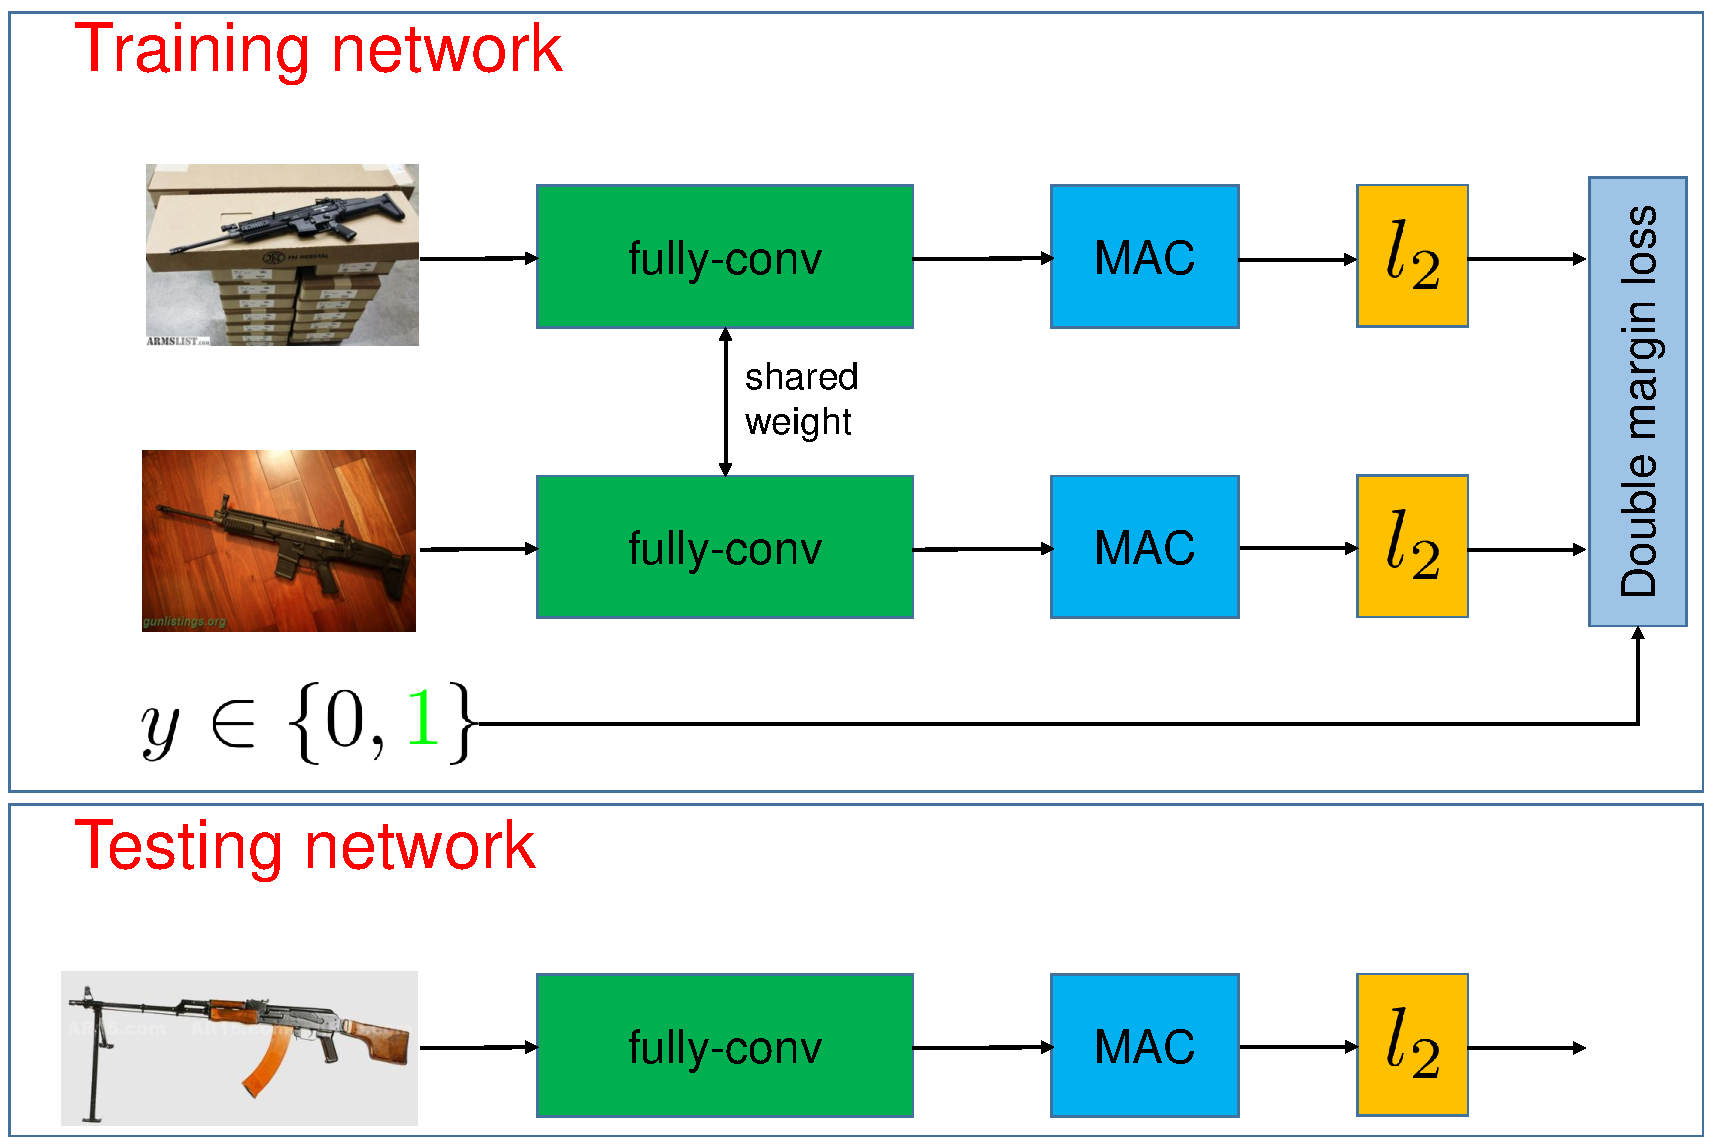
\includegraphics[width=0.95\linewidth]{chapter_double_margin_train_test_arch.pdf}
  \caption[基于双阈值对比损失方法的网络结构]{基于双阈值对比损失方法的网络结构,上面为训练网络,下面为测试网络}
  \label{fig:train_test_arch}
\end{figure}

\subsection{双阈值对比损失函数}
首先我们简要回顾传统的单阈值对比损失函数。给定图像对 $(I_p, I_q)$,以及对应的相似性标签 $y$ (如果两张图片是相似的,$y=1$,否则 $y=0$)。假如我们用 $f(I)$ 表示图片 $I$ 经过神经网络得到的特征,那么单阈值对比损失可以用如下的公式来表示

\begin{equation}\label{eq:single_margin_loss}
L(I_p, I_q) = \frac{1}{2}\left[yd^2 + (1-y)\max(\alpha - d, 0)^2\right]\, ,
\end{equation}

上式中,$d$ 是两个图像 $l_2$ 归一化特征之间的欧式距离($d= \lVert f(I_p)-f(I_q)\rVert_2$),$\alpha$ 是对不相似样本设定的一个阈值。单阈值对比损失函数试图把相似图像尽可能拉近,同时把不相似图像之间的距离推的超过设定的阈值 $\alpha$。

单阈值方法的一个明显缺点是网络在训练过程中会偏向相似图片对,因为相似图片对总是会贡献损失,除非相似图片之间的距离为 0。另外一个问题是,在实际训练过程中,很难为不相似图像对设定一个合适的阈值 $\alpha$,使得正负图片对贡献的损失是平衡的。总的来说,这两个问题都导致在实际中很难平衡正负样本贡献的损失,因而不能学习到很好的特征距离度量,导致学习到的模型在 Firearm14k 数据库上效果不佳。

为了缓解不平衡的损失问题,我们提出使用双阈值对比损失函数来优化网络模型。该损失函数可以用如下的公式表示

\begin{equation}\label{eq:double_margin_loss}
L(I_p, I_q) = \frac{1}{2}[y\max(d - {\alpha}_1, 0)^2 + (1-y)\max({\alpha}_2 - d, 0)^2]\, ,
\end{equation}

公式~\ref{eq:double_margin_loss} 中,$\alpha_1$ 和 $\alpha_2$ 是对应于相似与不相似图像对的阈值。很显然,为了使得损失函数有效且有意义,阈值不应该超过两个归一化的特征之间的距离的最大值(为 $\sqrt{2}$),因此下面的不等式成立

\begin{equation}
0 \leq \alpha_1 \leq \alpha_2 \leq \sqrt{2}\, .
\end{equation}

比较公式~\ref{eq:single_margin_loss} 与 \ref{eq:double_margin_loss},我们可以看出,单阈值与双阈值方法之间的差异主要在于相似图像对的损失如何计算:

\begin{itemize}
\item 单阈值方法:相似图像对总是会贡献损失
\item 双阈值方法:只有两张相似图像的特征距离大于阈值 $\alpha_1$ 的图像对才会贡献损失
\end{itemize}


当我们需要对模型的参数进行小幅度更新以取得更好的结果时,基于双阈值损失函数的方法尤其有效,我们将在实验部分对这种情况下的结果进行说明。我们在实验中发现,由于这种对相似样本更加「缓和」的损失,模型才能在分类任务的基础上继续提高检索的效果,具体实验结果见 \ref{subsec:double_margin_result_analysis}~节。

双阈值对比损失函数(公式~\ref{eq:double_margin_loss})中的两个阈值是该损失函数的核心,我们根据相似与不相似图像对的特征距离的分布来选择这两个阈值。由于数据库中图片数量庞大,可以组成的相似与不相似图像对的数目也十分庞大,因此不可能穷举所有组合,实际上,我们的做法是随机从训练集中采样大约 400000 对图像(相似图像对与不相似图像对的数目相等),并计算图像对特征距离,分别得到相似与不相似图像对特征距离的分布。然后我们把两个分布的均值作为选取两个阈值 $\alpha_1$ 和 $\alpha_2$ 的起点。

\subsection{两步训练策略}

我们在训练中使用的基础模型是从 ImageNet 数据集训练得到的分类模型,由于 ImageNet 数据库和我们的 Firearm14k 数据库差异非常大,Firearm14k 图像的特征不能很好地被基础模型所表达。为了解决这个问题,我们首先使用分类任务微调基础模型,经过分类任务微调以后,模型已经能够比较好地表达 Firearm14k 数据库中的图像特征,此时的检索性能已经较好。然后,我们使用分类微调后的模型,进一步使用我们提出的双阈值损失函数进行微调,实验表明,检索的结果会得到进一步的提升。

\subsection{特征降维}

当训练过程完成以后,我们进一步使用主成份分析法(PCA)对特征进行降维,因为 PCA 能够进一步提升特征的效果~\cite{Radenovic2016CNNIR,Babenko2014NeuralCF,Tolias2015ParticularOR,Babenko2015AggregatingLD}。在我们的实验中,我们使用了 PCA 方法,但是并未使用白化 (whitening),因为我们发现白化特征会引起检索效果的大幅度下降。

\section{实验}\label{sec:double_margin_exprt}
\subsection{评价指标}
在实验中,我们在训练集上训练模型,在验证集上采用 mAP 来选择合适的模型。我们使用两种评价指标来报告模型在测试集上的结果。第一种评价指标是 mean average precision (mAP),mAP 常用来衡量检索系统的总体性能。第二个评价指标是 Rank-k 准确率~\cite{Jgou2011ProductQF,Song2016DeepML},Rank-k 准确率计算的是在所有的查询图片中,其 $K$-邻近图片中存在至少一张同类图片的查询图片的比例。Rank-k 准确率注重于检索方法返回的前面的结果,在实际场景下,如图像搜索引擎及电商网站在线购物,用户更关心前面返回 $K$ 个结果,因此 Rank-k 准确率这个指标更加能够反映实际需求。

\subsection{实验设置}
我们使用了开源框架 PyTorch\footnote{\url{http://pytorch.org/}} 来实现我们的整个方法,我们使用的服务器搭载了英伟达 TITAN X(Pascal) GPU,显存容量为 12G,同时搭载两颗英特尔 Xeon 12 核 CPU。在实验中,我们所用的基础模型为 VGG16 模型~\cite{Simonyan2014VeryDC},该模型是在 ImageNet 分类数据库上训练得到的。针对我们的任务,我们对模型进行了一些修改,我们把模型的全连接部分去掉,只使用了该模型的全卷积部分。

我们使用了两步训练的办法对模型进行了训练,下面分别介绍这两步训练的过程。

\begin{enumerate}
\item 使用分类损失微调网络

在这个步骤中,我们使用了 Firearm14k 数据库中的训练集和验证集的所有 127 类图片,我们把这些图片分为训练和验证数据,比例为 70\% 和 30\%。我们在第 \ref{chapter:firearm_dataset}~章 \ref{sec:dataset_stats}~节已经提到过,该数据库类别高度不平衡,因此我们使用了加权的交叉熵损失函数来训练网络,对于某个样本来说,该损失函数形式如下:

\begin{equation}
l = -w_k \log\frac{\exp(x_k)}{\sum_{i=0}^{126} \exp(x_i)}
\end{equation}

上式中,$k$ 是该样本的真实类别,神经网络的输出为 127 个节点,$x_i$ 是神经网络在第 $i$ 个节点的输出值,$w_k$ 是第 $k$ 类对应的权重。我们使用的批(batch)大小为 128,训练过程(epoch)数量为 50,初始学习率(learning rate)为 0.001,冲量(momentum)为 0.9,权值衰减(weight decay)系数为 0.0005,学习率每过 30 个训练过程,减为之前的十分之一。

为了防止模型过拟合,我们也使用了数据增广~\cite{Krizhevsky2012ImageNetCW}(data augmentation),由于我们使用的网络可以接受不同大小的图像,因此我们在实验中保持图像长宽比不变,把图像的最长边缩放到 $[256, 384]$ 这个范围 (步长为 8),同时我们也使用了随机的水平翻转,随机的旋转以及随机的颜色变换(亮度,对比度等变化)。基础网络的分类微调过程,大约耗时 2 个小时。最后,我们选择在验证数据上分类准确率最高的模型,然后在这个模型基础上再进行第二步的训练。

\item 使用双阈值对比损失函数微调网络

正如 \ref{sec:double_margin_method}~节介绍的,使用 Siamese 结构的网络训练图像时,需要输入一对图像以及相应的标签,因此我们需要生成训练数据。对于 Firearm14k 训练集中的每一类图像,我们随机生成 180 对相似图像对以及 180 对不相似图像对。我们总共生成了 38520 对图像来训练第一步得到的网络模型。当然,对于神经网络来说,这样的训练数据量并不够,为了增加图像的多样性,增强模型的泛化能力,每 5 个训练过程,我们会重新生成一次训练图像对。在训练过程中,我们同样使用了数据增广方法,和分类训练数据增广方法一致,这里不再赘述。

由于输入网络的图像大小以及长宽比不同,我们无法使用传统的批处理(batch processing)的方法来输入图像,在训练过程中,我们每次输入一个图像对,然后反传误差,等输入网络的图像对达到 64 对时\footnote{所以可以认为我们使用的批大小是 64},我们对网络的参数进行一次更新。在验证集上,我们使用 mAP 衡量网络的性能,从而选择最佳的网络模型。我们使用随机梯度下降方法优化网络的参数,实验中使用的参数设置为:初始学习率为 0.001(每过 10 个训练过程变为原来的十分之一),冲量为 0.9,权值衰减为 0.0005。网络的最大训练过程为 30,整个训练大约需要 14 个小时的时间。
\end{enumerate}

\subsection{实验结果与分析}\label{subsec:double_margin_result_analysis}

本节介绍具体的实验,主要有单阈值与双阈值对比损失函数的比较与结果分析,两步训练的结果以及分析,以及双阈值函数中的两个阈值选取对检索性能的影响分析。

\begin{table}[t]
  \centering
  \caption{单阈值方法与双阈值方法的对比}
  \label{table:single_vs_double}
  \begin{tabular}{@{}lllllll@{}}
    \toprule
    \multirow{2}*{} & \multirow{2}*{方法} & \multirow{2}*{mAP(\%)} & \multicolumn{4}{c}{Rank-k 准确率(\%)} \\

    \cmidrule(lr){4-7}
    & & & k=1 & k=2 & k=4 & k=8 \\
    \midrule
    (a) & VGG  & 31.1 & 83.75 & 91.25 & 95.0 & 96.25 \\
    \midrule
    (b1) & retr-s & 35.1 & 80.0 & 86.25 &  92.5&  96.25\\
    (b2) & retr-d & 47.1 & 87.5 & 88.75 & 95.0 & 97.5 \\
    \bottomrule
  \end{tabular}
\end{table}

\textbf{(1)单阈值与双阈值对比损失函数的比较}

在本部分,我们评估了所提出的双阈值对比损失函数的有效性,和单阈值对比损失函数进行了比较。在我们的比较中,双阈值与单阈值方法使用了相同的基础模型(VGG16 模型)并且使用了相同的设置。对于两种方法,我们都进行了多轮实验,然后我们从多轮实验中选择效果最好的模型来比较这两个方法。我们在表~\ref{table:single_vs_double} 列出了两种方法在测试集上的实验结果,对于 Rank-k 准确率,我们使用了 $k=[1,2,4,8]$。在表~\ref{table:single_vs_double} 中,第一行「VGG」是使用原始 VGG 网络得到的结果,第二行「retr-s」代表使用单阈值对比损失函数得到的检索结果,第三行「retr-d」代表使用双阈值损失函数得到的结果。从这些结果,我们可以看出:

\begin{itemize}
\item 单阈值与双阈值方法都可以提高基础的 VGG 模型的 mAP。
\item 原始的 VGG 的模型已经在 Rank-k 准确率这个指标上取得了不错的效果,因而 Rank-k 准确率这个指标更加具有挑战性。基于双阈值损失函数的方法在这个指标上仍然有所提高,但是基于单阈值损失函数的方法在这个指标上反而比原始的 VGG 模型还要差。
\end{itemize}
总的来说,基于双阈值对比损失函数的方法在两种评价指标下的效果都优于传统的单阈值损失函数,双阈值损失函数在 mAP 指标上取得了 47.1\% 的结果,而单阈值方法只取得了 35.1\% 的结果,双阈值方法相对于单阈值方法整整提高了 34.2\% 的 mAP,而且没有额外的时间和内存等开销,这说明了双阈值损失函数的有效性。

我们也从直观上研究了为什么基于双阈值损失函数的方法更加有效。我们分别画出了基于双阈值函数的方法以及基于单阈值函数的方法,在一个训练过程中不同批数据中,相似样本对以及不相似样本对对整个损失的贡献率,所得到的结果如图~\ref{fig:img_pair_loss_contribution} 所示。图~\ref{fig:img_pair_loss_contribution} 上部分展示的是使用单阈值对比损失函数的结果,下部分展示的使用双阈值对比损失函数的结果。可以看出,使用单阈值损失函数时,刚开始训练时的一些批次数据,正样本对总的损失的贡献明显大于负样本对,这样的话,网络的训练可能会被引入错误的方向,导致后续模型优化出现方向错误,因而检索效果很差;使用双阈值损失函数,从训练一开始,正负样本贡献的损失与负样本贡献的损失相对平衡,因而网络优化方向更好,检索的效果也更好。

\begin{figure}[t]
  \centering
  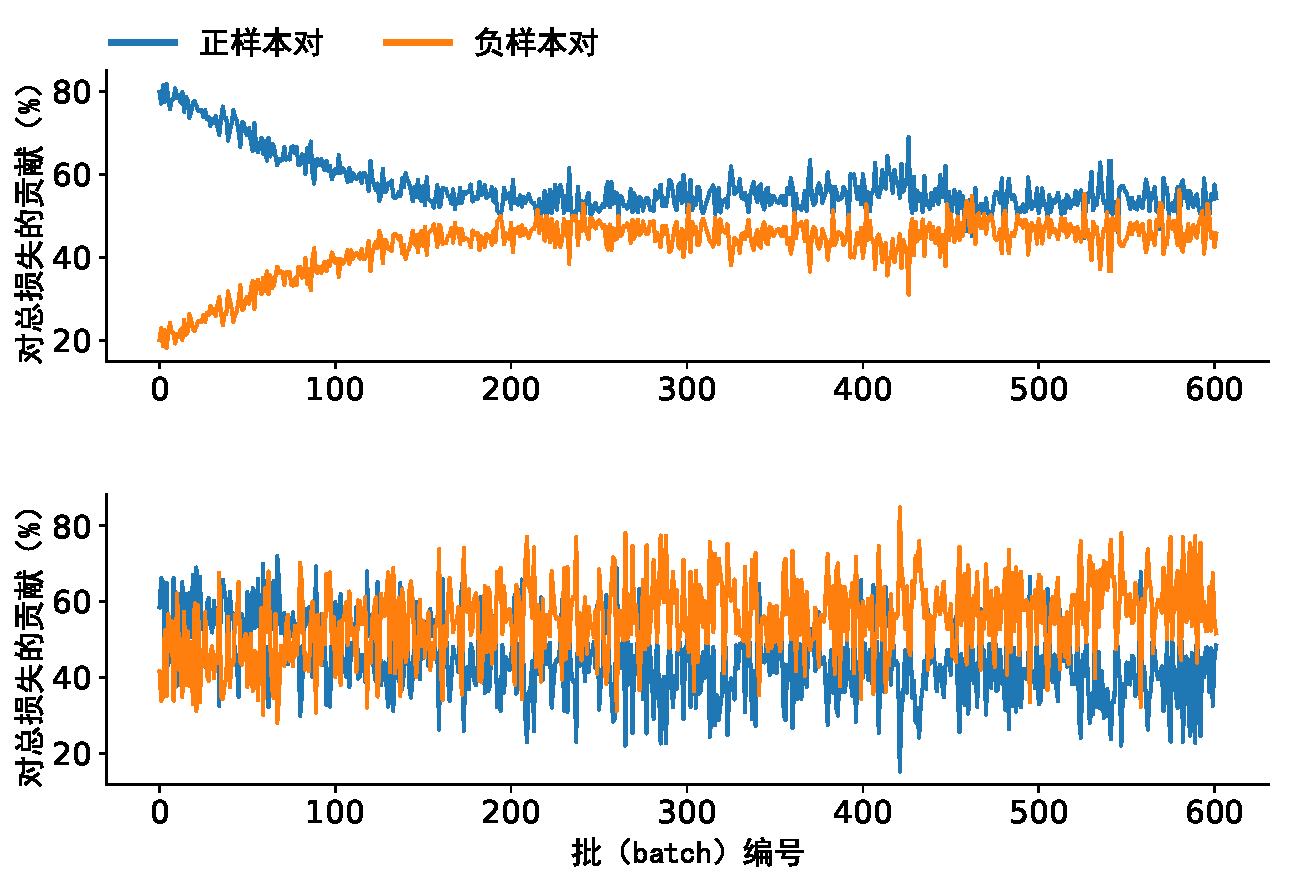
\includegraphics[width=0.95\linewidth]{chapter_double_margin_pos_neg_loss_contrib.pdf}
  \caption[使用不同损失函数时,正负样本对对损失的贡献率]{使用不同损失函数(\textbf{上图}:单阈值对比损失函数,\textbf{下图}:双阈值对比损失函数),一个训练过程中不同批次数据,相似样本对与不相似样本对对总体损失的贡献率}
  \label{fig:img_pair_loss_contribution}
\end{figure}

\begin{table}[t]
\centering
 \caption{两步训练策略的结果}
 \label{table:two_step_training}
	\begin{tabular}{@{}lllllll@{}}
		\toprule
		\multirow{2}*{} & \multirow{2}*{方法} & \multirow{2}*{mAP(\%)} & \multicolumn{4}{c}{Rank-k 准确率(\%)} \\

		\cmidrule(lr){4-7}
		& & & k=1 & k=2 & k=4 & k=8 \\
		\midrule
		(a) & VGG  & 31.1 & 83.75 & 91.25 & 95.0 & 96.25 \\
		\midrule
		(b1) & Cls & 65.4 & 92.5 & 96.25 & 97.5 & 98.75 \\
		(b2) & Cls + retr-s & -- & -- & -- & -- & -- \\
		(b3) & Cls + retr-d &  68.4 & 95.0 & 98.75 &98.75 & 100.0 \\
		\bottomrule
	\end{tabular}
\end{table}

\textbf{(2)两步训练策略的效果}

我们进一步研究了两步训练策略的有效性。首先我们使用分类任务(采用加权的交叉熵损失)来微调网络的参数,然后我们在分类微调得到的模型基础上,再使用双阈值对比损失函数进行优化。我们将实验的结果列在表~\ref{table:two_step_training} 中,「Cls」表示使用分类任务训练得到的结果,「Cls + retr-s」代表先使用分类任务后使用单阈值损失函数得到的结果,「Cls + retr-d」代表先使用分类任务后使用双阈值损失函数得到的结果。

从实验结果,我们可以看出,仅仅通过在分类任务上训练模型,在 mAP 这个指标上,我们得到的模型相对于基础的 VGG 模型已经取得了 110.2\% 的效果增强。我们发现,在分类微调的模型基础上,在使用单阈值对比损失函数无法进一步提高模型的检索效果,但是使用双阈值对比损失函数微调模型,无论在 mAP 还是 Rank-k 准确率的指标上都可以进一步提高网络的检索效果。实际上,我们发现,如果使用单阈值方法,无论我们设定阈值为多少,随着训练过程的进行,模型的性能会持续下降(因此在表~\ref{table:two_step_training} 中,我们没有列出「Cls + retr-s」的结果)。这种情况是可以预见的:因为模型经过分类任务的微调,当我们再使用检索任务微调模型的参数时,必须要小心,使用单阈值的方法将会使得模型优化向错误的方向前进(因为单阈值方法中,相似图像对的损失占上风)。正是由于使用双阈值损失函数,正负样本贡献的损失更加平衡,所以模型的检索效果得到进一步提升。

\begin{figure}[t]
	\centering
	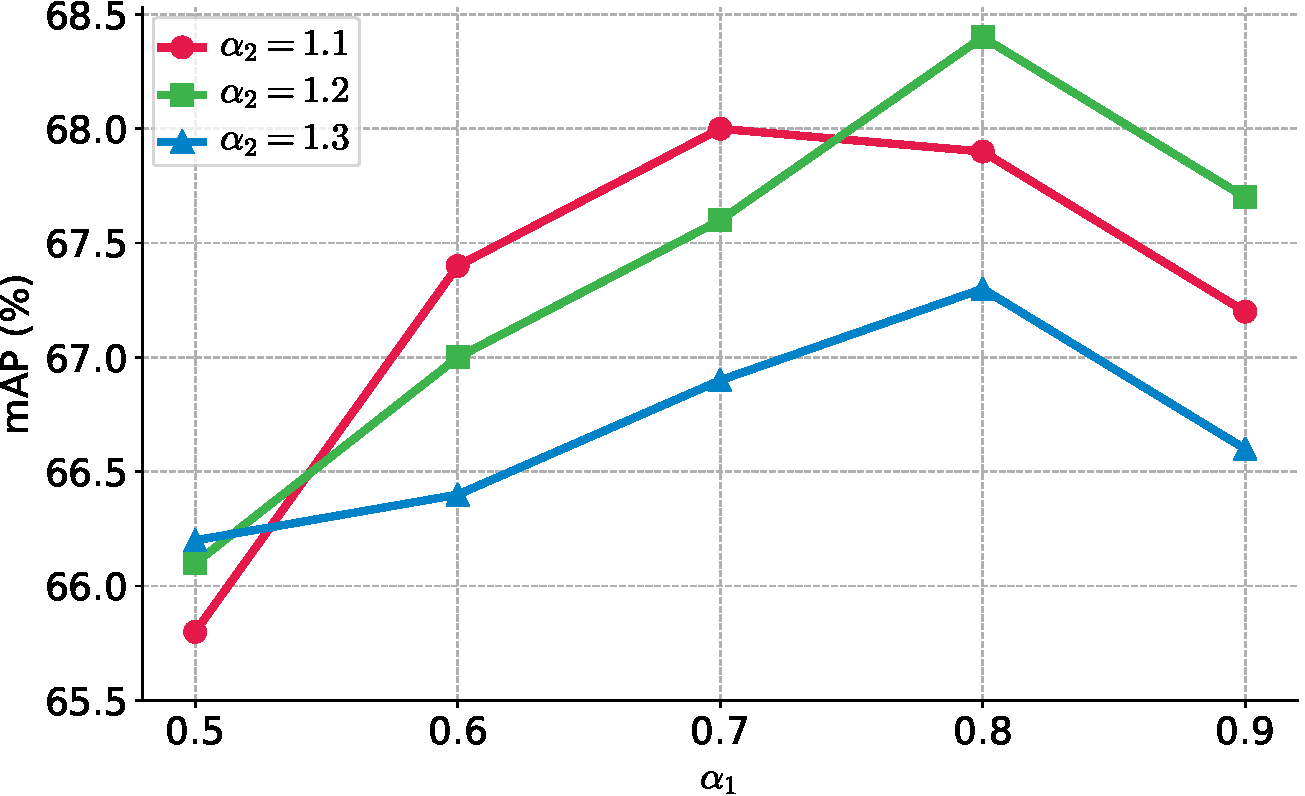
\includegraphics[width=\linewidth]{chapter_double_margin_impact_of_margins.pdf}
	\caption{双阈值对比损失函数中两个阈值对模型检索性能的影响}
	\label{fig:impact_of_margins}
\end{figure}

\textbf{(3)阈值选取及对检索结果的影响}

在本部分,我们将讨论双阈值损失函数中的两个阈值 $\alpha_1$,$\alpha_2$ 对模型检索效果的影响。正如在 \ref{sec:double_margin_method} 节讨论的那样,我们使用在分类任务上微调好的模型(因为检索的模型是在分类模型的基础上进行优化的),从训练数据集采样图像对,然后计算图像对中两幅图像的特征之间的距离,然后画出相似图像对与不相似图像对特征距离的分布曲线。这两个分布曲线近似为正太分布,具体例子可以参见图~\ref{fig:feat_dist_distribution_change} 中的某一张图。我们把两个分布的均值作为阈值选择的起点,对于相似和不相似图像对,两个分布均值分别为 0.9 以及 1.2。图~\ref{fig:impact_of_margins} 展示了两个阈值对模型检索性能的影响(以 mAP 指标来衡量)。从图上可以看出,两个阈值的选取应该在分布的均值附近选择,才能取得比较高的检索结果,另外,两个阈值之间的间隔非常重要,这个间隔不能太「松弛」(也就是说 $\alpha_2 - \alpha_1$ 太小),也不能太「紧」($\alpha_2 - \alpha_1$ 太大),无论间隔太大或者太小,都会影响模型的性能。最终,我们选择设定 $\alpha_1=0.8$ 以及 $\alpha_2=1.2$ 来优化我们的模型。

\begin{figure}[t]
	\centering
	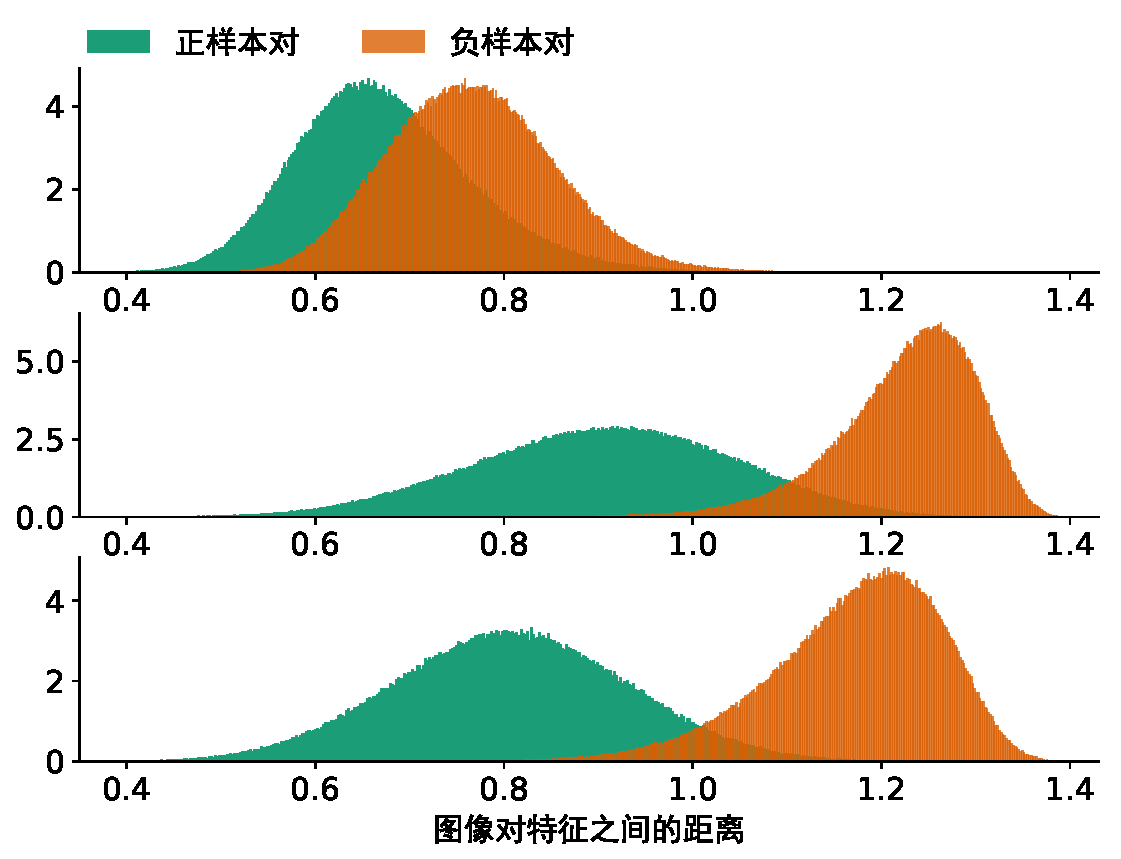
\includegraphics[width=\linewidth]{chapter_double_margin_dist_distribution_change.pdf}
	\caption{不同模型下相似与不相似图像对特征距离的概率分布}
	\label{fig:feat_dist_distribution_change}
\end{figure}

\subsection{检索效果的可视化}
在本部分,我们将采用可视化的方式来帮助我们理解为什么所提出的方法能够取得更好的效果。我们比较了三种不同的模型,第一种是原始的 VGG16 模型,第二种是在 Firearm14k 数据库使用分类任务微调以后的模型,第三种是在分类模型基础上继续使用双阈值损失函数微调的模型。我们随机采样了大约 500000 相似与不相似图像对,然后我们分别使用了不同模型计算相似与不相似图像对特征距离。图~\ref{fig:feat_dist_distribution_change} 展示了不同模型下,正负样本对特征距离的分布曲线。对于原来的 VGG 模型(图~\ref{fig:feat_dist_distribution_change},\textbf{上图}),相似图像对与不相似图像对的图像特征距离分布重合非常大,因此模型输出的特征对于判断两个图像是否是相似有很大的不确定性,所以检索结果较差(31.1\% mAP)。经过在分类任务上的微调,我们得到了第二个模型(图~\ref{fig:feat_dist_distribution_change},\textbf{中图}),相似与不相似图像对的特征距离分布之间的重叠大幅减少,因此模型的检索精度也有了很大的提升(检索的 mAP 为 65.4\%)。当我们进一步在分类模型基础上使用双阈值损失函数对模型进行微调后,我们得到了最终的模型(图~\ref{fig:feat_dist_distribution_change},\textbf{下图}),我们可以看到特别是相似图像对的特征距离分布发生了明显的变化:分布曲线的形状发生了变化,相对于中图的「矮胖」,变得更加「高瘦」。分布的变化也带来了检索结果的进一步提升(检索 mAP 68.4\%)。在图~\ref{fig:double_margin_retrieval_result} 中,我们也展示了一些采用我们的方法得到的检索结果,从这些结果我们可以看出,当枪支图片只占据图像的一小部分时候,我们的方法可以准确找到相似的图片(第 2 个和第 7 个检索结果),另外我们的方法对于枪支的姿态角度变化也具有较强的鲁棒性。

\begin{figure}[t]
	\centering
	\includegraphics[width=\linewidth]{chapter_double_margin_retrieved_results_more.pdf}
	\caption{我们的方法的一些示例检索结果}
	\label{fig:double_margin_retrieval_result}
\end{figure}


\begin{figure}[t]
	\centering
	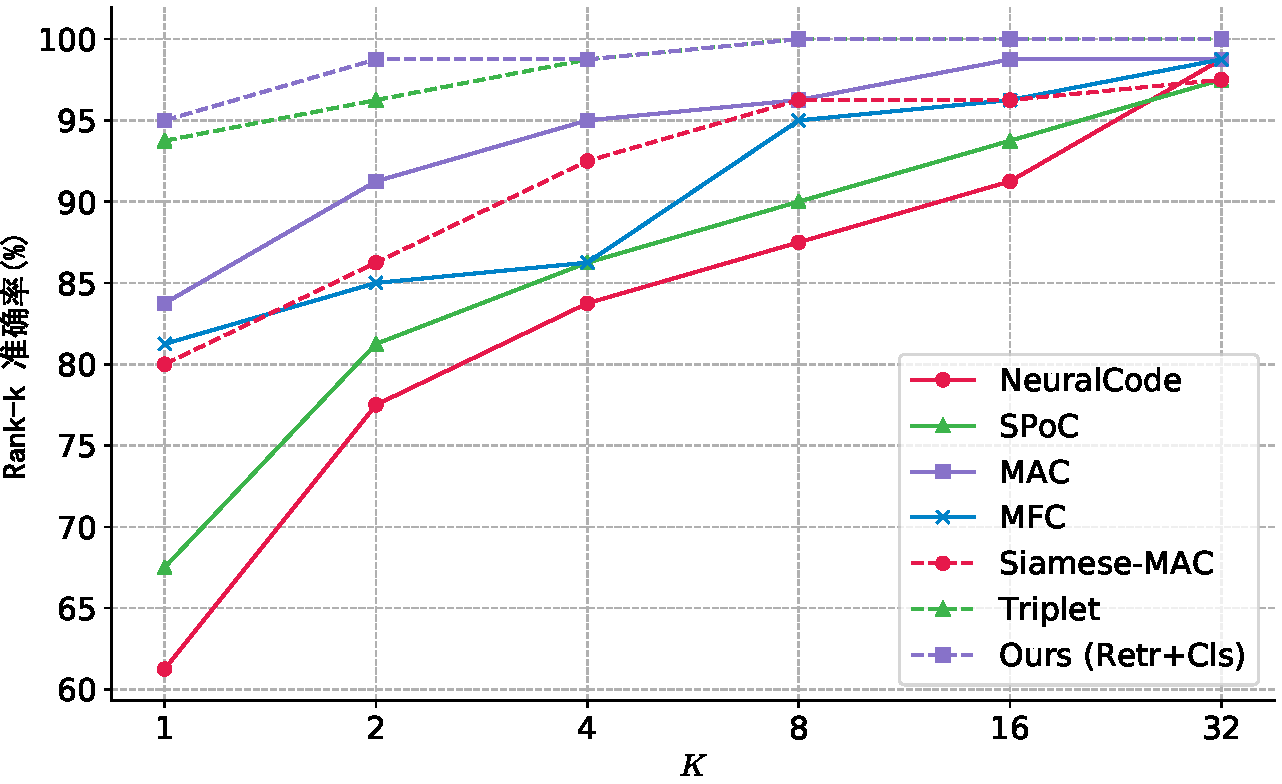
\includegraphics[width=\linewidth]{chapter_double_margin_compare_rank_k_accu.pdf}
	\caption{不同方法 Rank-k 准确率的比较(\%)}
	\label{fig:rank_k_accuracy_compare}
\end{figure}

\begin{table}[!t]
  \centering
  \begin{threeparttable}
    \caption{与其他主流方法的结果比较}
  \label{table:firearm_retrieval_compare_with_soa}
  \begin{tabular}{@{}lllllll@{}}
    \toprule
   \multirow{2}*{方法} & \multicolumn{6}{c}{特征维度}\\
    \cmidrule(lr){2-7}
     & D=512 & D=256 & D=128 & D=64 & D=32 & D=16\\
    \midrule
    Neural codes~\cite{Babenko2014NeuralCF} & 15.9 & 15.8 & 15.7 & 14.6 & 13.7 & 10.5\\
    SPoC~\cite{Babenko2015AggregatingLD} & 23.3 & 23.4 & 23.1 & 22.4 & 20.6 & 18.4\\
    MFC~\cite{Hao2017MFCAM} & 30.0 & 29.8 & 29.5 & 28.0 & 24.5 & 20.9 \\
    MAC~\cite{Tolias2015ParticularOR} & 36.1 & 36.4 & 36.5 & 35.4  & 32.3 & 27.8\\
    \midrule
    Siamese-MAC~\cite{Radenovic2016CNNIR} & 35.6 & 36.2 & 37.2 & 37.3 & 35.2 & 31.4\\
    TripletNet\textsuperscript{$\dagger$}~\cite{Gordo2016DeepIR} & 67.98 & 68.57 & 69.60 & 69.97 & 68.1 & 60.67\\
    \midrule
    Ours (retr-d) & 45.79 & 46.17 & 46.61 & 46.75 &45.36 & 42.03 \\
    Ours (cls) & 66.57 & 67.2 & 68.53 & 68.67 & 67.47 & 59.99\\
    Ours best (cls + retr-d) & \textbf{68.63} & \textbf{69.15} & \textbf{70.14} & \textbf{70.07} & \textbf{68.48} & \textbf{61.59}\\
    \bottomrule
  \end{tabular}
  \begin{tablenotes}
      \footnotesize
      \item \textsuperscript{$\dagger$} TripletNet 的权重是也由 Firearm14k 分类微调的模型初始化的。
  \end{tablenotes}
  \end{threeparttable}
\end{table}

\subsection{与其他方法的对比}
在本节,我们比较了所提出的双阈值方法与其他主流方法的检索结果,这些方法中,有的方法使用的是未经过微调的模型(称为 off-the-shelf 模型),另外一些方法使用的是经过微调的模型。为了保证对比的公平性,所有的方法都由我们使用 VGG16 模型实现。对于那些基于 off-the-shelf 模型的方法~\cite{Babenko2014NeuralCF,Tolias2015ParticularOR,Babenko2015AggregatingLD,Hao2017MFCAM},我们根据论文中所给的设置来实现对应的方法,在这些方法中,MFC 是我们在第 \ref{chapter:mfc}~章提出的多尺度全卷积的方法。对于那些使用模型微调的方法~\cite{Gordo2016DeepIR,Radenovic2016CNNIR},我们使用了和我们的方法尽可能一致的设置,然后在 Firearm14k 数据库上训练模型。按照惯例~\cite{Babenko2015AggregatingLD,Radenovic2016CNNIR},从这些方法得到的图像特征都经过 $l_2$ 归一化,然后经过了 PCA 变换,最后再一次经过 $l_2$ 归一化处理。

首先,我们报告不同的方法在 mAP 指标上的结果,所有的实验结果参见表~\ref{table:firearm_retrieval_compare_with_soa}。这里的结果表明,off-the-shelf 模型(表~\ref{table:firearm_retrieval_compare_with_soa},\textbf{上部})的 mAP 分数都相对较低,这是由于 Firearm14k 数据库和 ImageNet 数据库的巨大差异,这些预训练的模型无法生成具有区分性的特征,因而检索效果并不理想。使用单阈值方法微调的模型~\cite{Radenovic2016CNNIR}表现也不理想,使用三元组损失的 TripletNet~\cite{Gordo2016DeepIR}的表现相对单阈值方法提高了很多。最后,我们的提出的方法在不同的特征维度下都超过了其他方法。值得注意的是,我们的方法在特征维度被压缩到极低的情况下仍然表现良好,例如当特征维度为 16 时,检索的 mAP 仍然达到了 61.59\%。

我们也计算了不同方法在 Firearm14k 测试集上的 Rank-k 准确率,在这个实验中,我们使用的是 512 维特征,得到的实验结果如图~\ref{fig:rank_k_accuracy_compare}所示。从图中可以看出,当 $k$ 比较大时($k=16$ 或 $k=32$ 时),各种方法的 Rank-k 准确率都较高,这说明 Rank-k 指标是比较容易的指标;当 $k$ 比较小时,SPoC~\cite{Babenko2015AggregatingLD},NeuralCode~\cite{Babenko2014NeuralCF} 和 Siamese-MAC~\cite{Radenovic2016CNNIR} 等方法,表现较差,TripletNet 方法~\cite{Gordo2016DeepIR} 和我们的方法此时表现较好,特别是我们的方法,在 $k=1$ 或 $k=2$ 时,表现要优于 TripletNet 方法。

\section{本章小结}\label{sec:double_margin_conclusion}
在本章中,我们详细介绍了提出的双阈值对比损失函数,我们提出该方法的动机主要有两个,一是目前单阈值对比损失函数无法保证正负图像对在训练时贡献的损失的平衡,二是我们提出的 Firearm14k 数据库与 ImageNet 数据库之间的巨大差异导致直接微调模型效果欠佳。我们提出使用双阈值对比损失函数来解决模型训练过程中正负图像对贡献的损失不平衡的问题,同时提出使用两步训练的策略来解决数据库之间图像差异大的问题。在实验部分,我们把提出的方法与当前的主流方法进行了比较,并给出可视化的分析,证明我们的方法为什么有效,实验结果表明我们的方法在不同的特征维度下检索效果都超过了当前的主流方法。

%!TEX root = ../Thesis.tex

\chapter{工作总结与展望}\label{chapter:conclusion}

从深度卷积神经网络在 2012 年的兴起~\cite{Krizhevsky2012ImageNetCW} 到图像检索领域的研究者将卷积神经网络与图像检索的技术结合起来~\cite{Babenko2014NeuralCF,Gong2014MultiscaleOP} ,再到最近基于卷积神经网络的方法在一些常用数据库上的效果已经超过了传统的方法~\cite{Gordo2016DeepIR,Noh2017LargeScaleIR},短短四五年时间,基于卷积神经网络的方法在图像检索领域已经取得了巨大的进步。本文的工作也是围绕卷积神经网络在图像检索领域的应用展开的,我们研究了影响从神经网络提取的特征的有效性的因素,希望能够提出对物体的形状,位置,姿态等的变化更加鲁棒的检索算法,同时结合了对与敏感图像目标检索的需求,下面对本文的的工作做一总结,并对未来工作进行展望。

\section{工作总结}
本文围绕卷积神经网络在图像检索领域的应用,分析了目前方法的优缺点,并且结合对敏感图像识别的需求,开展了相关的工作,主要工作总结如下:

\textbf{1. 本文建立了一个大规模的枪支图像数据库}

在社交网络上,大量的枪支图片会引起用户不适,也有可能引起暴力行为的增加,需要适当的控制与处理。目前的基于深度卷积神经网络的检索方法,在模型的训练过程中都需要大量的训练数据,否则模型将过拟合。这些都要求一个数据量丰富的数据库,从而方便研究者开展该方面的研究,但是目前并没有一个大规模的枪支图片数据库存在。为了这样的需求,我们构建了一个大规模的枪支图像数据库,该数据库包含 14755 张来自 167 类不同类型枪支的图片,可以为枪支图片精细分类与检索等研究提供所需的数据基础。

\textbf{2. 本文提出了一种多尺度全卷积的图像实例检索方法}

在工作中,我们发现目前基于卷积神经网络的图像检索方法在提取图像特征时,并未详细分析影响提取的特征有效性的因素,采用的设置都是一些比较随意的选择,因此我们通过实验详细分析了三个重要因素对提取的特征有效性的影响,这三个因素分别是:输入神经网络的图像尺寸,多尺度特征表达以及 PCA 和白化矩阵的学习方式。结合我们的实验和分析,我们提出了一种多尺度全卷积的图像实例检索方法,我们的方法在多个数据库上都取得了良好的检索效果。

\textbf{3. 本文提出了一种基于双阈值对比损失函数的敏感目标检索方法}

在当前的社交网络上,大量的枪支图片的出现,要求社交媒体的监管者对这些图片进行适当的管理,在取证科学中,也有大量需要鉴定枪支图片类型的需求,这些问题都可以通过图像检索相关的技术得到有效解决。在本工作中,我们研究了微调卷积神经网络进行敏感目标检索的可行性,我们以枪支图片作为一个具体的应用场景,我们发现,传统的单阈值对比损失函数对于枪支图像检索,存在一定的缺点:第一,使用该函数,在模型的训练过程中,正负样本贡献的损失不平衡,模型的训练偏向正样本对;第二,由于枪支数据库与训练基础 CNN 模型的 ImageNet 数据库存在巨大的域差异,直接使用这些模型针对检索任务微调,并不能取得良好的检索精度。我们提出使用双阈值对比损失函数解决网络训练中正负样本贡献的损失不平衡的问题。我们采用两步训练的策略缓和域差异带来的性能下降问题,第一步,我们在 Firearm14k 上针对分类任务微调网络,第二步再针对检索任务(使用双阈值对比损失函数)微调模型。在 Firearm14k 测试集上,我们把提出的方法与其他主流方法进行了对比,实验结果表明,我们的方法在不同特征维度上的检索准确率都要优于其他主流方法。

\section{工作展望}
虽然我们的方法在图像检索任务上取得了不错的结果,但是该领域仍有许多没有完全解决的问题,未来的工作将关注以下几个问题:

\textbf{1. 利用显著性分析或注意力机制解决图像中小物体检索的问题}

在我们的工作中,我们发现基于卷积神经网络的方法,在图像中的物体尺寸非常小的情况下,效果并不理想,因为卷积神经网络提取的是图像的全局特征,并不像 SIFT 特征描述子一样提取的是局部特征。包含小物体的图像,如果使用卷积神经网络提取特征,特征中可能包含了大量周边环境的特征,对小物体的检索造成了干扰。目前的很多检索方法只是希望通过模型的训练,使得模型能够隐式地关注目标物体区域,并没有去显示学习目标物体的位置,因此,我们可以结合一些显著性分析~\cite{Zhao2015SaliencyDB,Li2016DeepCL,Wang2015DeepNF}或者注意力机制的方法~\cite{Song2017DeepSA,Xiao2015TheAO,Zheng2017LearningMC},自动检测图像中可能的物体,然后提取显著性区域的特征,忽略周边环境的干扰,从而增强小物体图像检索的有效性。

\textbf{2. 研究基于深度学习的局部特征描述特征}

深度学习提取的特征本质上是图像全局信息的表达,特别是网络经过多层卷积与池化以后,特征图中一个元素在原图上对应着很大一片区域(感受野比较大),无法像传统的 SIFT 特征一样,进行空间几何校验,进行检索结果重排序,提高检索的准确率。目前这方面的工作还比较少,Noh 等~\cite{Noh2017LargeScaleIR} 提出的方法就是试图学习深度局部特征,但是他们使用的训练方法并未针对检索的任务,局部特征有效性有待提高,因此这方面的研究也是未来的一个方向。

\textbf{3. 研究基于特征量化和哈希的精细图像检索问题}

在本文中所使用的图像特征都是实值特征,并不是二值化的特征,在检索数据库规模较小的情况下,这些方法是可行的,但是当数据库规模巨大(亿级别或者十亿级别)时,这样的方法弊端是明显的,一方面特征存储需要消耗大量空间,另外计算特征之间的相似度也会消耗大量时间,达不到实时性的要求。目前哈希方法使用的数据库都是一些粗糙类别层次的数据库,如 CIFAR10\footnote{\url{https://www.cs.toronto.edu/~kriz/cifar.html}},NUS-WIDE~\cite{Chua2009NUSWIDEAR},并不是精细类别的数据库,因此基于特征量化或者深度学习的图像特征哈希编码学习也是一个非常重要的研究方向。

\begin{figure}[!t]
\centering
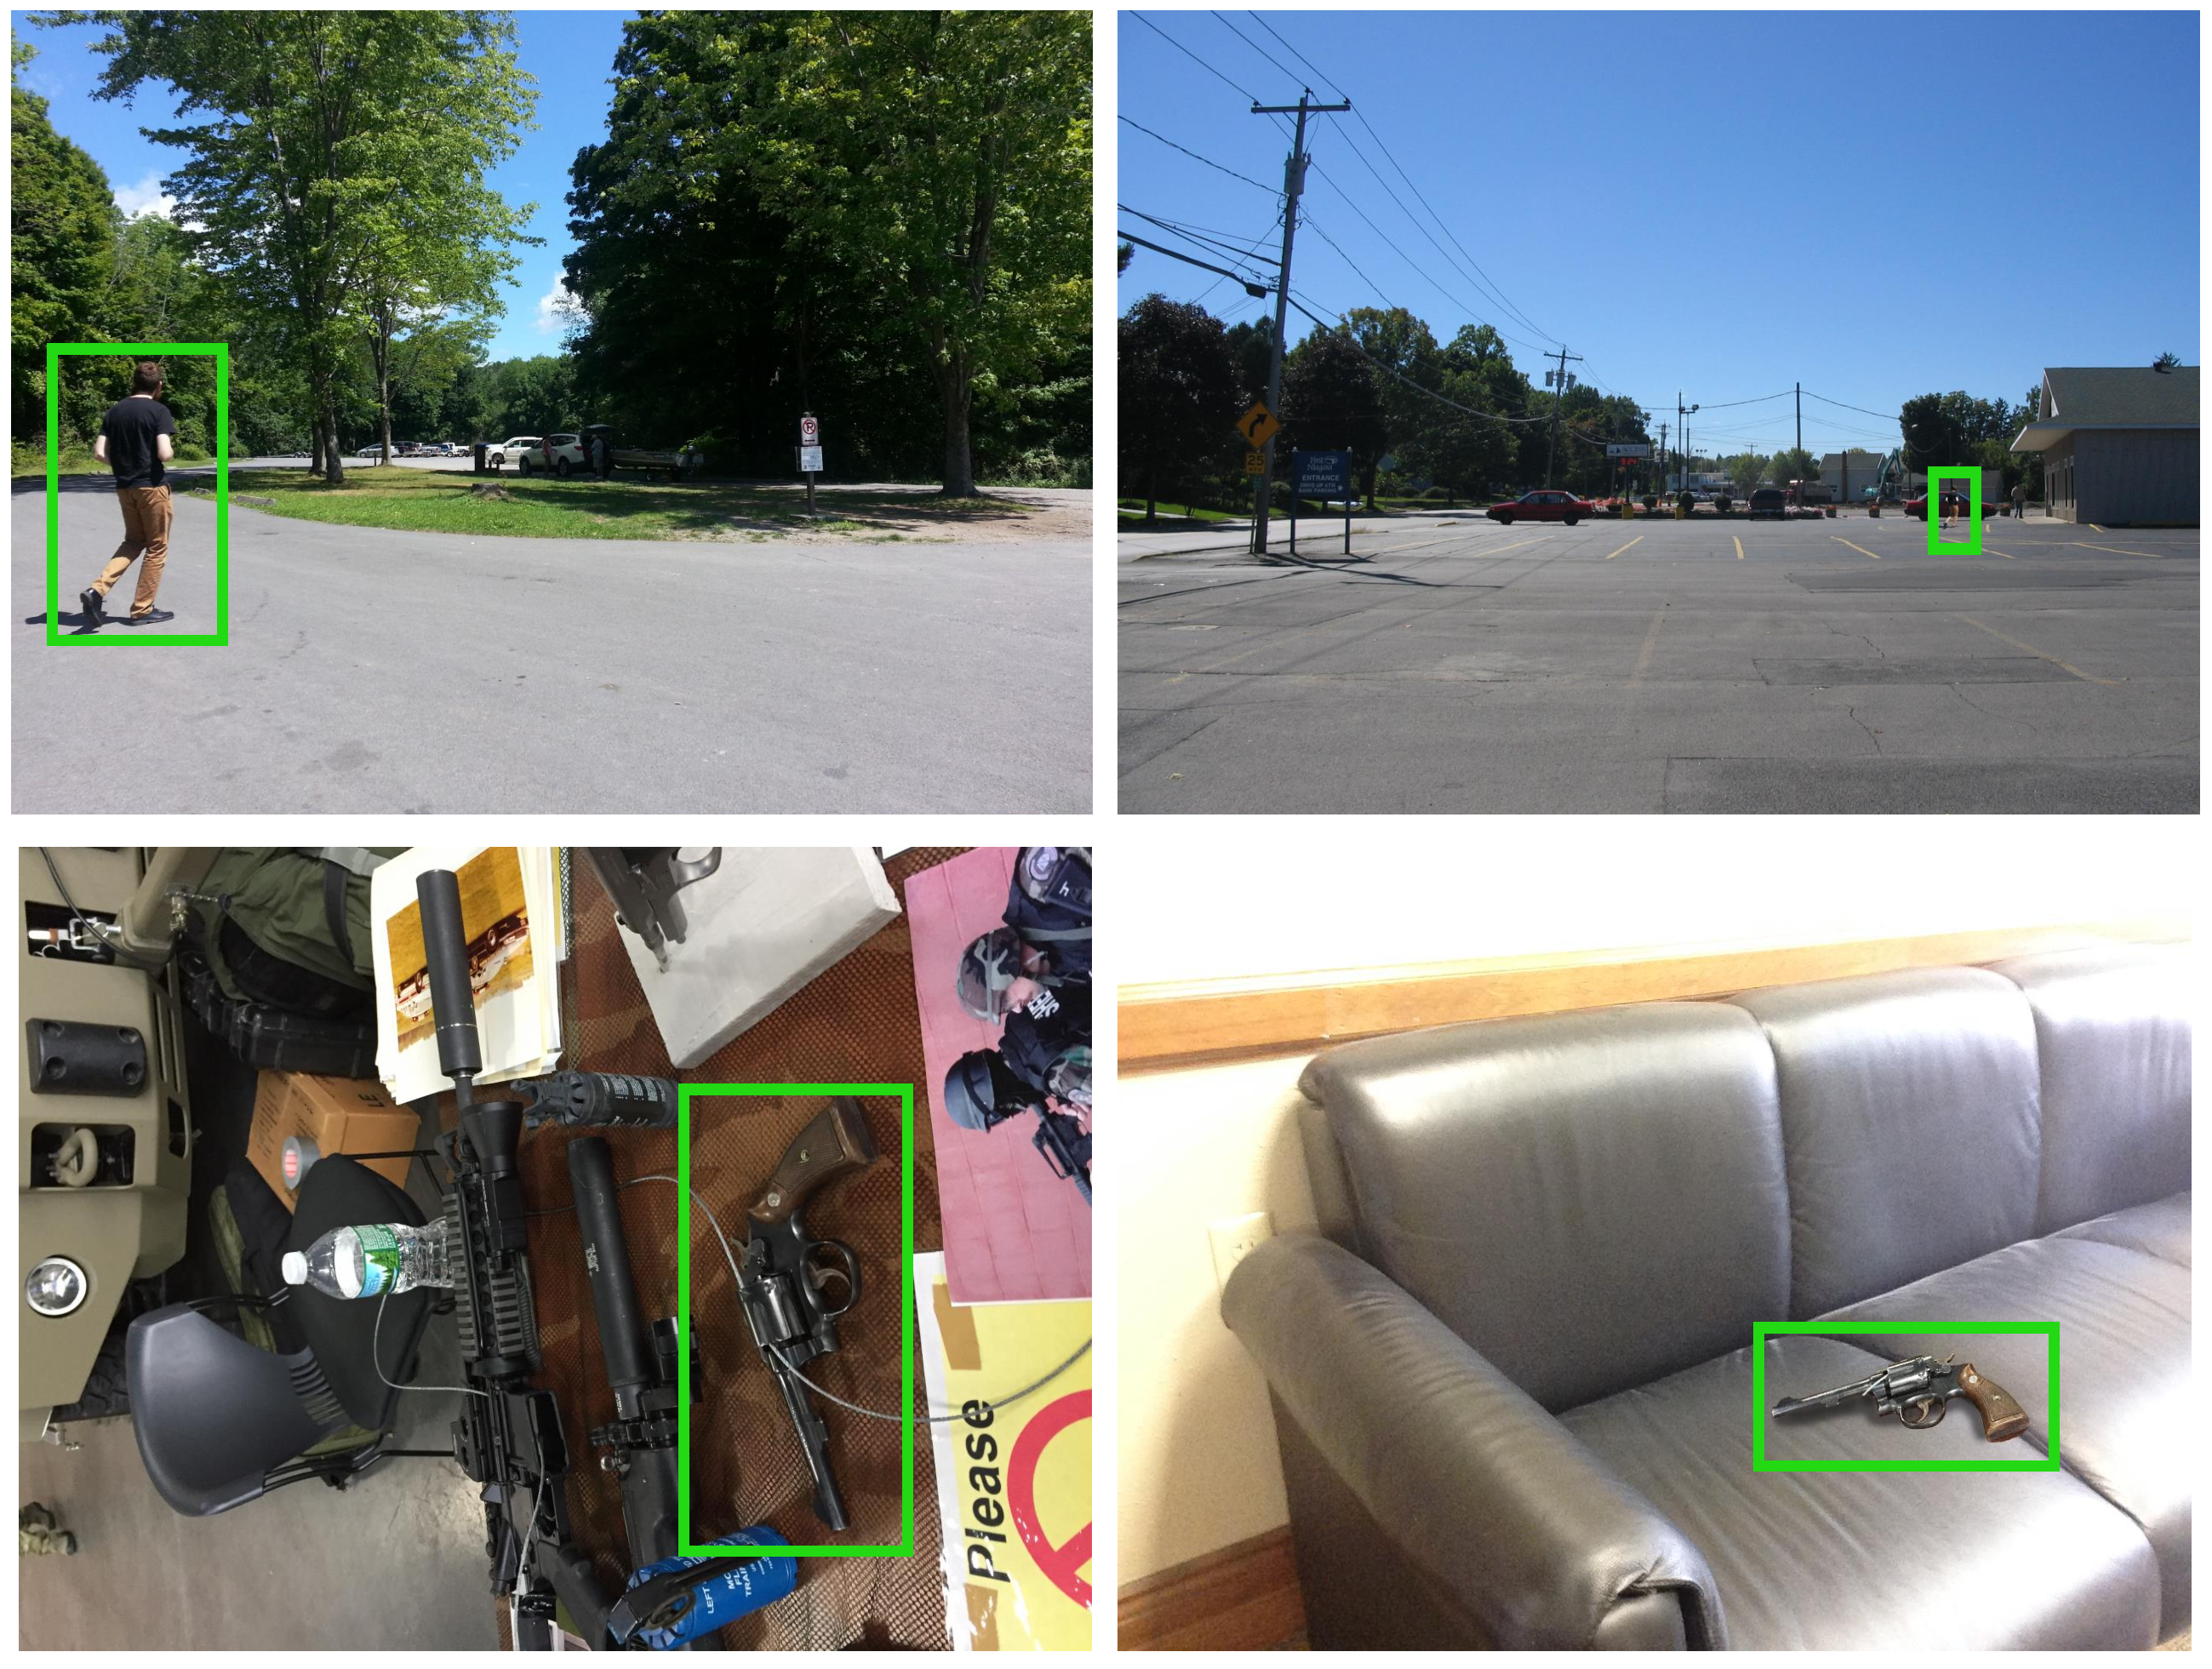
\includegraphics[width=\linewidth]{chapter_conclusion_forensic_retrieval.pdf}
\bicaption[两个图片剪切篡改的实例]{两个图片剪切篡改的实例(\textbf{左}:donor 图片;\textbf{右}:剪切拼接后图片)}{Two examples of image splicing (Left: donor image; Right: spliced image)}
\label{fig:forensic_image_retrieval}
\end{figure}

\textbf{4. 利用图像检索的方法解决图像取证的问题}

随着数字图像技术的发展,图像伪造技术也不断进步,网络上以及媒体上出现了各种伪造的照片。在图像取证中,有一类图片伪造方法是剪切拼接(splicing)~\cite{Farid2009ImageFD,Cozzolino2015SplicebusterAN,Iuliani2015ImageSD},也就是把一张图片(称为 donor 图片)一部分剪切拼接到另一张图片上(称为 base 图片),达到欺骗目的,图~\ref{fig:forensic_image_retrieval} 展示了两例剪切拼接的实例(图相框中是对应的相同物体)。如果能通过图像检索技术找到剪切后的图像中物体的原图,那么就可以很容易判断该图像是被篡改过的,因此基于图像检索的技术也能在图像取证领域中发挥一定的作用。






%%% ++++++++++++++++++++++++++++++++++++++++++++++++++++++++++++++++++++++++++++++++++
% main content
%-
%-> Appendix
%-
\cleardoublepage%
% \appendix% initialize the environment
% 
\chapter{中国科学院大学学位论文撰写要求}

学位论文是研究生科研工作成果的集中体现,是评判学位申请者学术水平、授予其学位的主要依据,是科研领域重要的文献资料。根据《科学技术报告、学位论文和学术论文的编写格式》(GB/T 7713-1987)、《学位论文编写规则》(GB/T 7713.1-2006)和《文后参考文献著录规则》(GB7714—87)等国家有关标准,结合中国科学院大学(以下简称“国科大”)的实际情况,特制订本规定:\url{http://onestop.ucas.edu.cn/home/info/abc167cb-4589-4e05-b014-052fa9291d0c/1}。
% appendix content
%-
%-> Backmatter: bibliography, glossary, index
%-
\backmatter% initialize the environment
\intotoc{\bibname}% add link to contents table and bookmark
\bibliography{Biblio/reference}% bibliography
%!TEX root = ../Thesis.tex

\chapter{致\quad谢}
% \chapter{致 谢}
在此论文完成之际,感谢中科院自动化所智能感知与计算研究中心为我的学习科研提供的软硬件环境,感谢导师的指导,感谢实验室的各位老师,同学以及工作人员等对我的帮助!

另外,感谢我的朋友们对我的支持,感谢我的父母对我的支持。

\chapter{作者简历及攻读学位期间发表的学术论文与研究成果}

\section*{作者简历:}

\noindent 2010 年 9 月 -- 2014 年 6 月,在中南大学信息科学与工程学院,获得学士学位。

\noindent 2014 年 9 月 -- 2018 年 7 月,在中国科学院自动化研究所攻读硕士学位。

\section*{已发表(或正式接受)的学术论文:}

\begin{enumerate}

	\item \textbf{HAO J}, WANG W, DONG J, et al. MFC: A multi-scale fully convolutional approach for visual instance retrieval[C]//2017 IEEE International Conference on Multimedia and Expo Workshops (ICMEW), 2017: 513 -- 518

	\item \textbf{HAO J}, DONG J, WANG W, et al. DeepFirearm: Learning Discriminative Feature Representation for Fine-grained Firearm Retrieval[C]//The 24th International Conference on Pattern Recognition (ICPR 2018), 2018
\end{enumerate}

\section*{申请或已获得的专利:}

\begin{enumerate}
	\item 谭铁牛,王伟,董晶,郝杰东.基于目标体图像的目标体检索方法、系统及装置。已申请
\end{enumerate}

\section*{参加的研究项目:}

\begin{enumerate}
	\item 国家自然科学基金:“基于迁移学习的图像隐写分析新方法研究”,项目编号:U1536120

	\item 国家自然科学基金重点项目:“应对大数据分析的情景融合个性化隐写理论与方法”,项目编号:U1636201

	\item 国家自然科学基金青年科学基金项目:“基于成像环境约束的低质量图像篡改取证研究”,项目编号:61502496

	\item 国家重点研发计划项目:“群体视觉大数据的透彻感知关键技术”,项目编号:2016YFB1001003

	\item 北京市自然科学基金项目:“基于深度学习的数字图像取证研究”,项目编号:4164102

	\item 国家自然科学基金重点项目:“具有强泛化能力的通用图像隐写检测技术研究”,项目编号:U1736119

	\item 国家自然科学基金面上项目:“基于深度对抗学习的隐蔽通信新方法研究”,项目编号:61772529

\end{enumerate}

% other information
\end{document}
%---------------------------------------------------------------------------%

